\chapter{Methods}
\label{Methods}
\section{Project Overview}
To help complete this Master thesis, I created various tools that would help create the final model outputs. 
The project is divided into three logical parts. 

\subsection{Part 1: Graphical User Interface (GUI) Tool}
The first part involves the development of a GUI tool to create and edit the network topography of interactions. 
This tool allows users to quickly and intuitively define agents, interaction parameters, environmental parameters and setting parameters. 
It provides functionalities for adding, editing, and visualizing nodes and edges, as well as importing and exporting the network structure. 
The tool created a network graph which is then used for part 2 and part 3. 

\subsection{Part 2: Simulation Framework}
The second part focuses on the simulation framework. 
The user provides an ODE model and the network topography as an input to the framework. 
The framework uses numerical solvers to simulate the interactions of the network over time.
As output, the user receives two outputs.
The first output is an array of time values that the solver used to calculate the population count. 
The second output is an array containing the population count of every agent. 

\subsection{Part 3: Analysis and Visualization}
The third part involves analyzing and visualizing the simulation results. 
The user can use a dashboard built using Plotly Dash to interact with the solver and network. 
The user can change parameter, environment values, and setting values on the fly. 
This allows for the user to quickly change parameter values and test different situations. 
The dashboard includes various starter plots that allows for the user to test the model. 

\section{Network Topography of Interactions}
In a microbial environment, there are numerous interactions occurring between agents. 
However not every agent can and will interact with one another.
Based on which agents interact with one another, a network topography can be created, capturing the dynamics of the interactions.
Every node represents a unique agent. 
An edge links agents together if there is an interaction occurring between the agents.  
The network allows for self-loops. 

Each node contains attributes and properties intrinsic to that agent. 
For example, this would include the starting population or concentration, reproduction speed (if any), or death rate (if any). 
Each edge likewise also contains attributes to capture the unique dynamic interactions between the agents. 
This could be the probability for a successful interaction, the burst size of a specific phage-bacteria pair, or the bacteria consumption rate of resources. 
Adding the attributes to the nodes and edges allow for the capture of various interaction dynamics within the context of the community. 
The interactions between the agents can be visualized and edited using a GUI tool. \newline 

A GUI tool has been developed using Python and NetworkX to help aid in the development of this network topography. 
With this tool, a network topography can be created by adding any number of agents of varying type, such as bacteria, phages, or resources.
There is an environment node that is used to store global environmental data, for example the temperature of the system, the pH of the system, washout rate, etc.
There is a settings node that holds information such as simulation length, max timestep, and type of ODE solver to use. 
The attributes of the agents, interactions, and environment can easily be edited using the GUI tool. \newline 

\Cref{fig:ss:initial_startup_GUI_tool} shows the layout of the very simple tool build using tkinter, matplotlib, and NetworkX %TODO: Citation needed. 
Although the button labels are self-explanatory, the buttons allow the user to add exactly 1 node of either type “P” for phage, “B” for bacteria, or “R” for resource and provide a name. 
That is however tedious for large graphs, so the user can add multiple nodes at the same time. 
The newly created node is provided with default parameter values that the user has to provide beforehand. 
This can be done by importing the tool as one would import any other Python package. 
The user provides a base class, extending the class of the tool. 
The user can proceed to override the default implementation of the method that gives the default value. 
It is of course possible to add single or multiple edges at once, remove edges, edit node and edge attributes, and import or export the graph. 

\begin{figure}
    \centering
    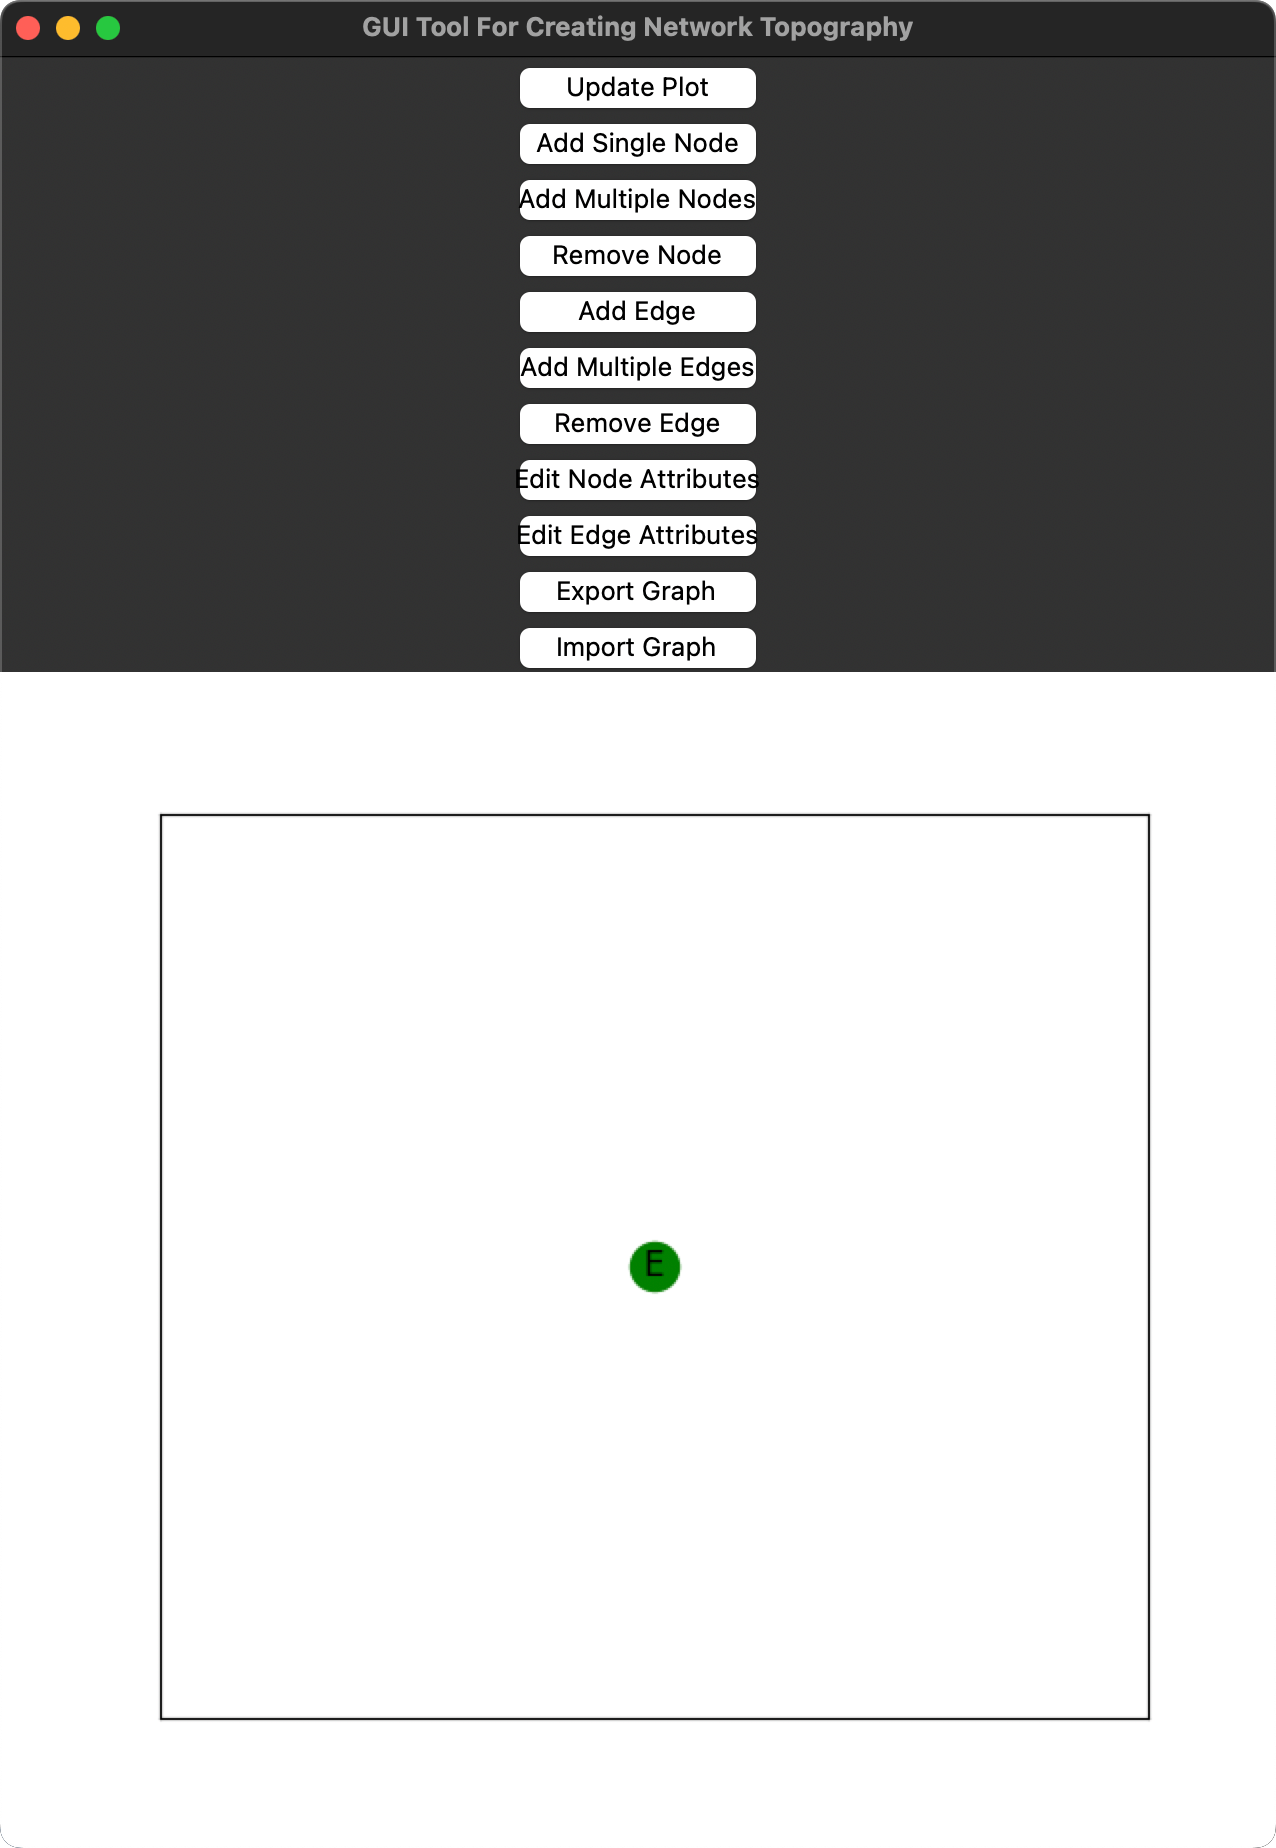
\includegraphics[width=0.5\linewidth]{Screenshots/initial_startup_GUI_tool.png}
    \caption{
        The GUI tool when you start up the program. 
        There are numerous tools that you can use to edit the graph. 
        By default, an environment node holding parameters such as pH and temperature is added. 
        A settings node is added as well, holding settings data to be used for the solver like the type of solver (RK23 or RK45). 
    }
    \label{fig:ss:initial_startup_GUI_tool}
\end{figure}


\begin{figure}
    \centering
    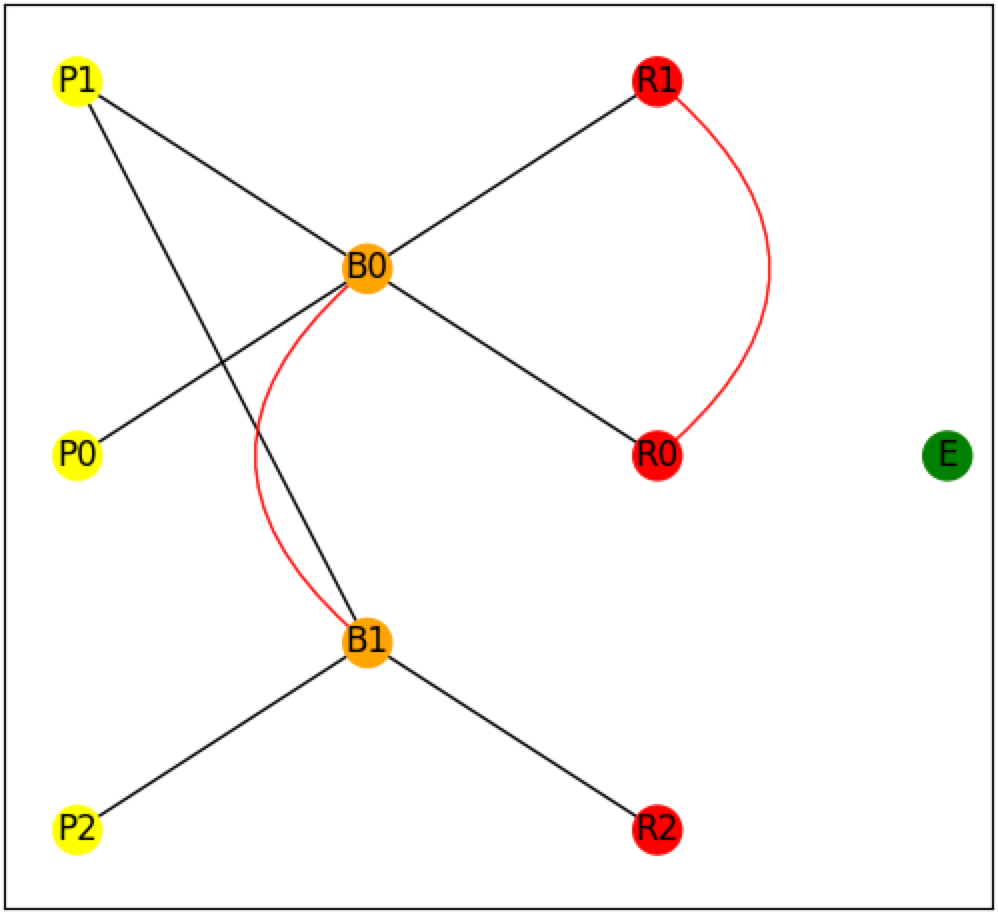
\includegraphics[width=0.5\linewidth]{Screenshots/example_network.png}
    \caption{
        An arbitrary $3\times2\times3$ network. Phage 0 (P0) interacts with bacteria 0 (B0). 
        P1 interacts with B0 and B1, etc. Finally, resource 0 (R0) interacts with R1 (an example of this would be a complex sugar degrading into a simple sugar over time). 
        The nature of the interaction needs to be defined and captured in the parameter names, values, and ODE equations. 
        It is up to the user to correctly define the interaction in the ODE model. 
        Nothing can interact with the environment and setting node, they are simply there to hold data about the environment and network solver.
    }
    \label{fig:ss:example_network}
\end{figure}
 

\section{Dashboard}
The dashboard allows for the user to interact with the network, the model, and some prebuilt visualizations, and is built into three logical sections. 
The first section allows for the user to edit the network parameters and setting values on the fly to quickly iterate through different conditions and to fine tune parameter selection without having to rebuild the network using the GUI tool. 
The second section allows for the user to see how the population count evolves over time for a given initial condition and parameter values, allowing to quickly test the network input. 
The final section allows for the user to run more advanced analysis on the network, for example by changing multiple parameter values and visualizing the output. 


\subsection{Editing Network and Parameter Values}
\label{sec:editing_network_and_parameter_values}
The editing network and parameter value section five sections. 
\subsubsection{Initial Condition}
The initial condition settings panel (\Cref{fig:ss:ds:initial_condition}) allows for the user to edit the initial starting values of the agents. Each agent type has their own table contianing the initial condition. 
\begin{figure}
    \centering
    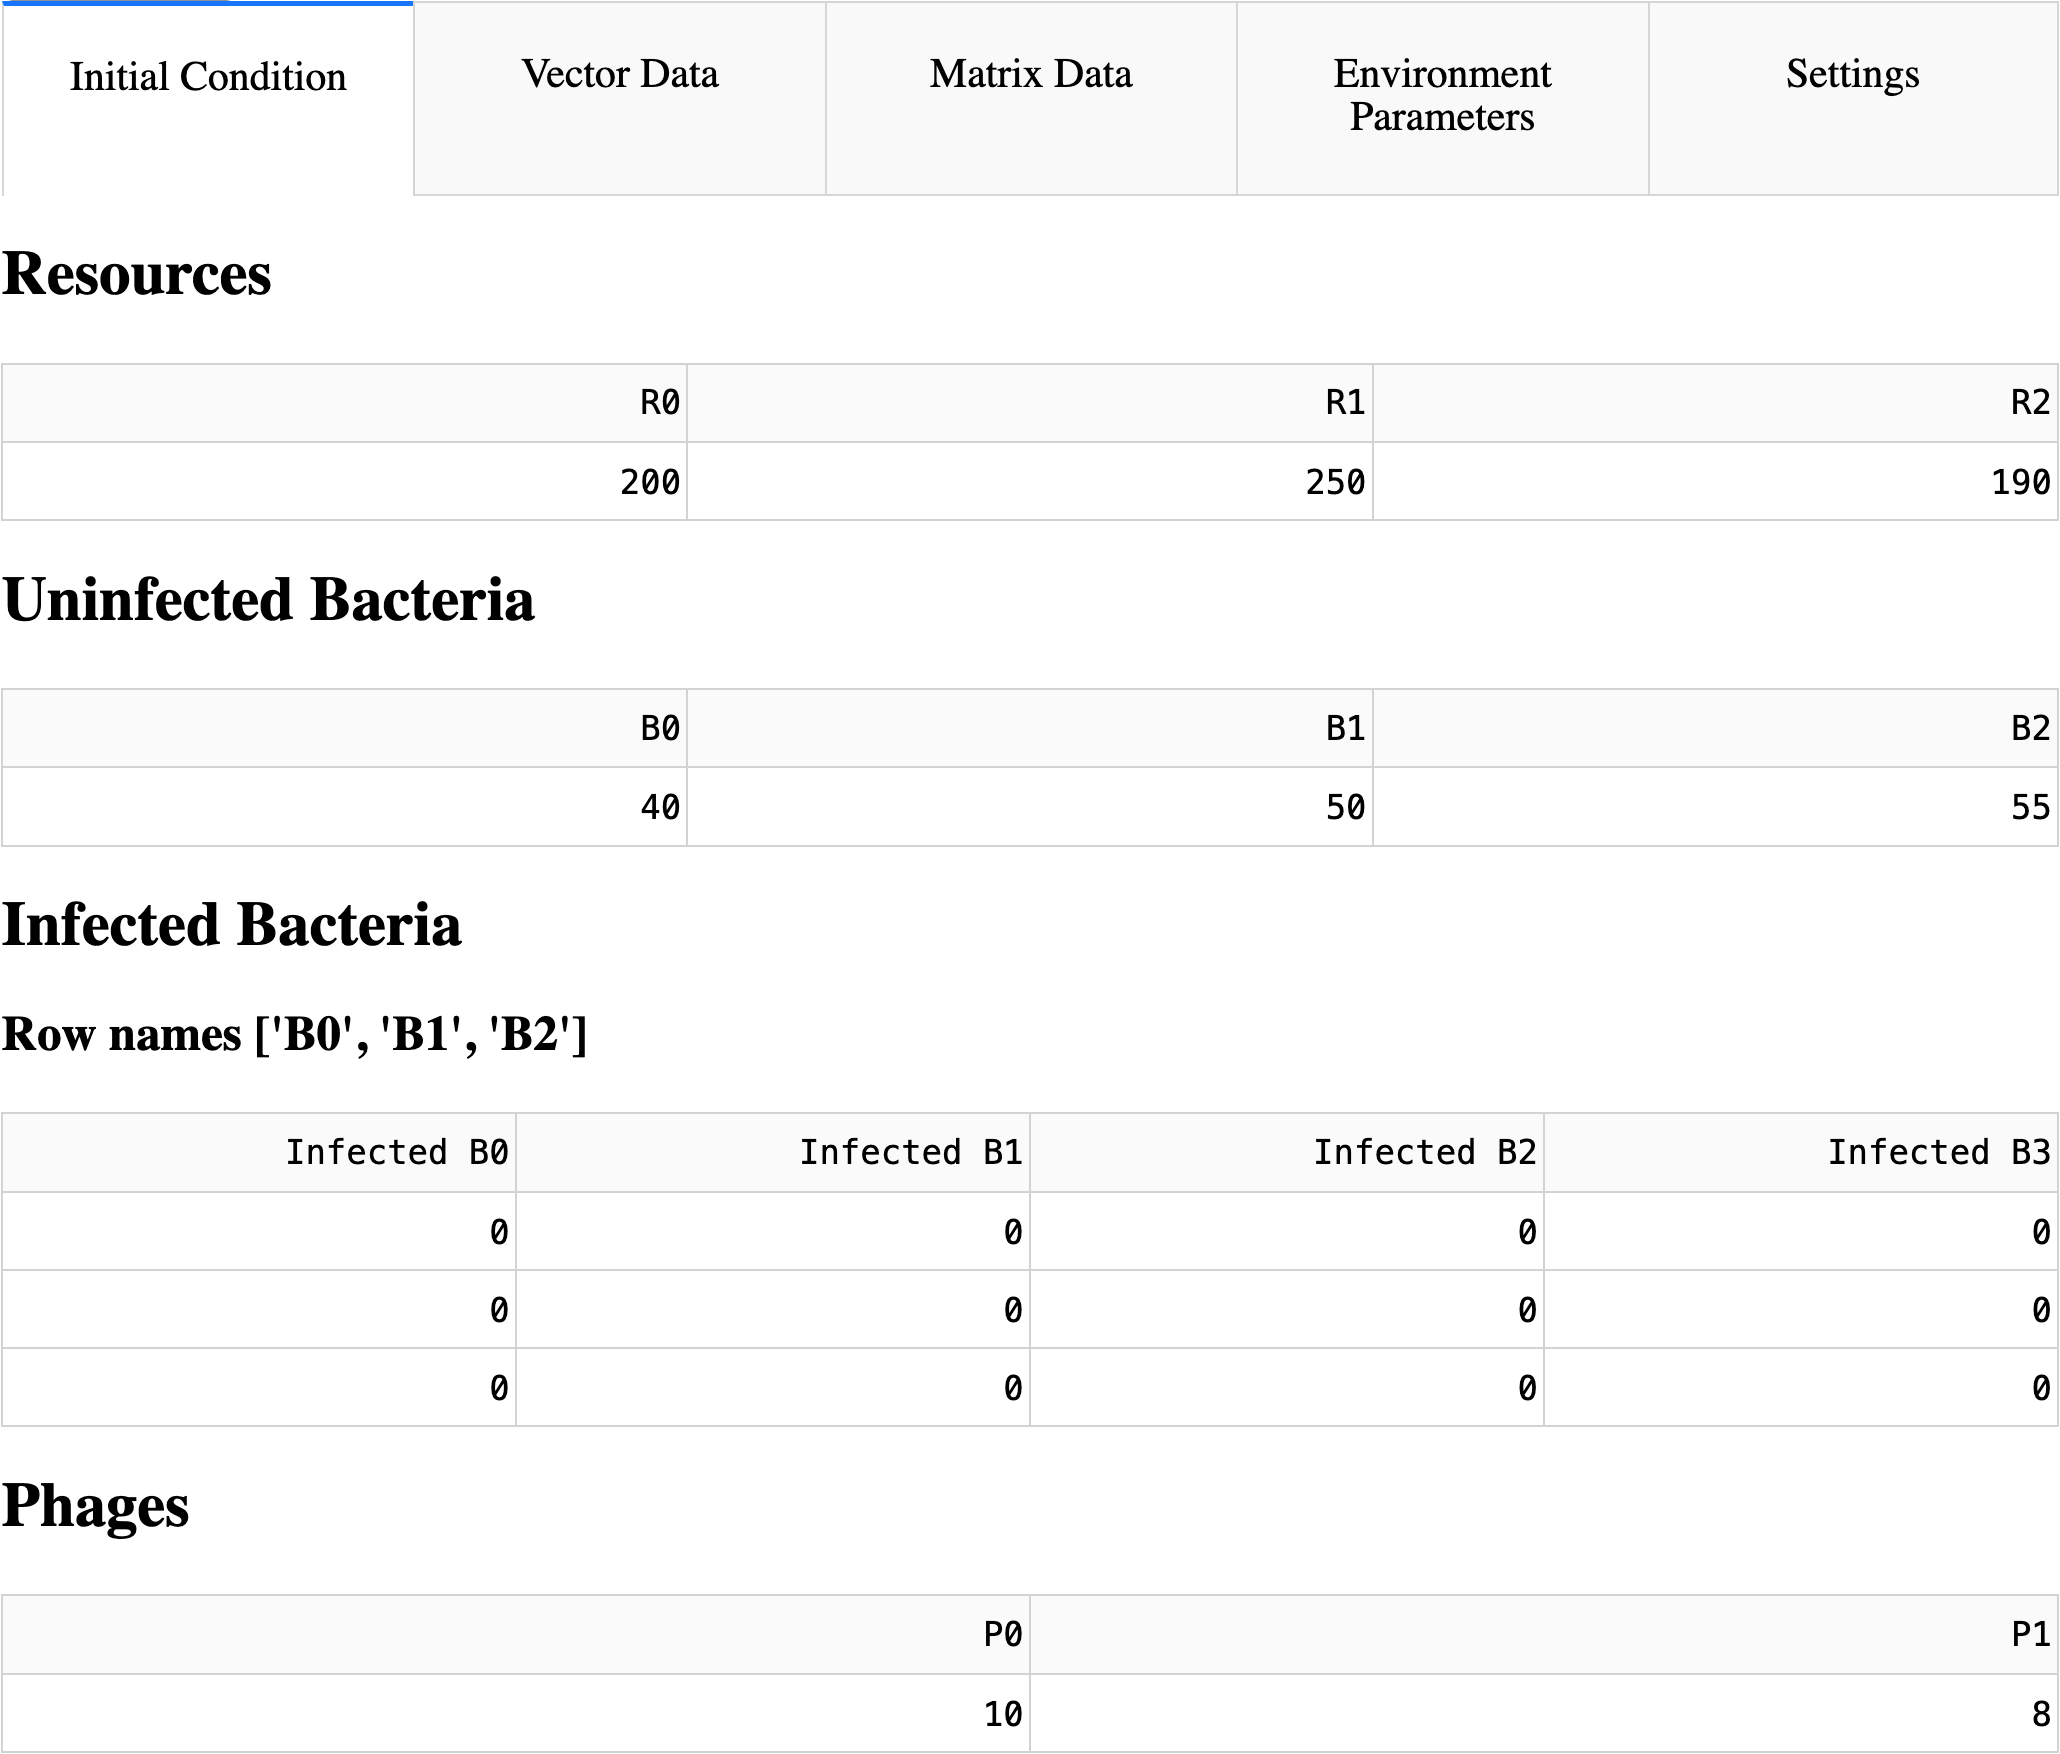
\includegraphics[width=1\linewidth]{Screenshots/DashboardSettings/initial_condition_settings.png}
    \caption{
        The panel where a user can edit the initial conditions of the agents. 
        The columns of each table show for which agent the value corresponds to. 
        A copy of this data is sent to the solver. 
        This instance of the model models a 3 resource, 3 bacteria, and 2 phage system. 
        The bacteria are split into an uninfected and an infected stage. 
        Once infected by a phage, a bacterium will go through four intermediary infection stages before lysing. 
        The infected stages are represented as a matrix, with each row representing a bacterial agent while each column represents the stage of infection. 
    }
    \label{fig:ss:ds:initial_condition}
\end{figure}

\begin{figure}
    \centering
    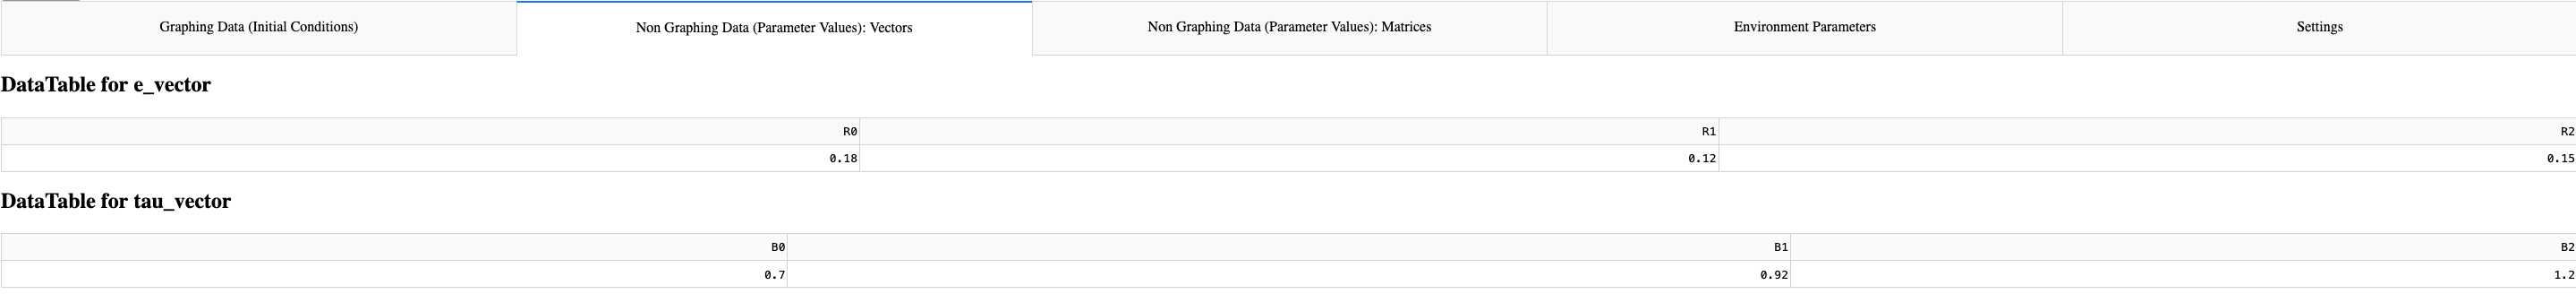
\includegraphics[width=1\linewidth]{Screenshots/DashboardSettings/initial_vector_settings.png}
    \caption{
        The panel where the user can edit the attributes for a given attribute name. 
        This version is specifically used represent the attributes that are associated with nodes, and are represented as a vector. 
        The columns of each table show for which agent the value corresponds to. 
        A copy of this data is sent to the solver.
    }
    \label{fig:ss:ds:vector}
\end{figure}
\begin{figure}
    \centering
    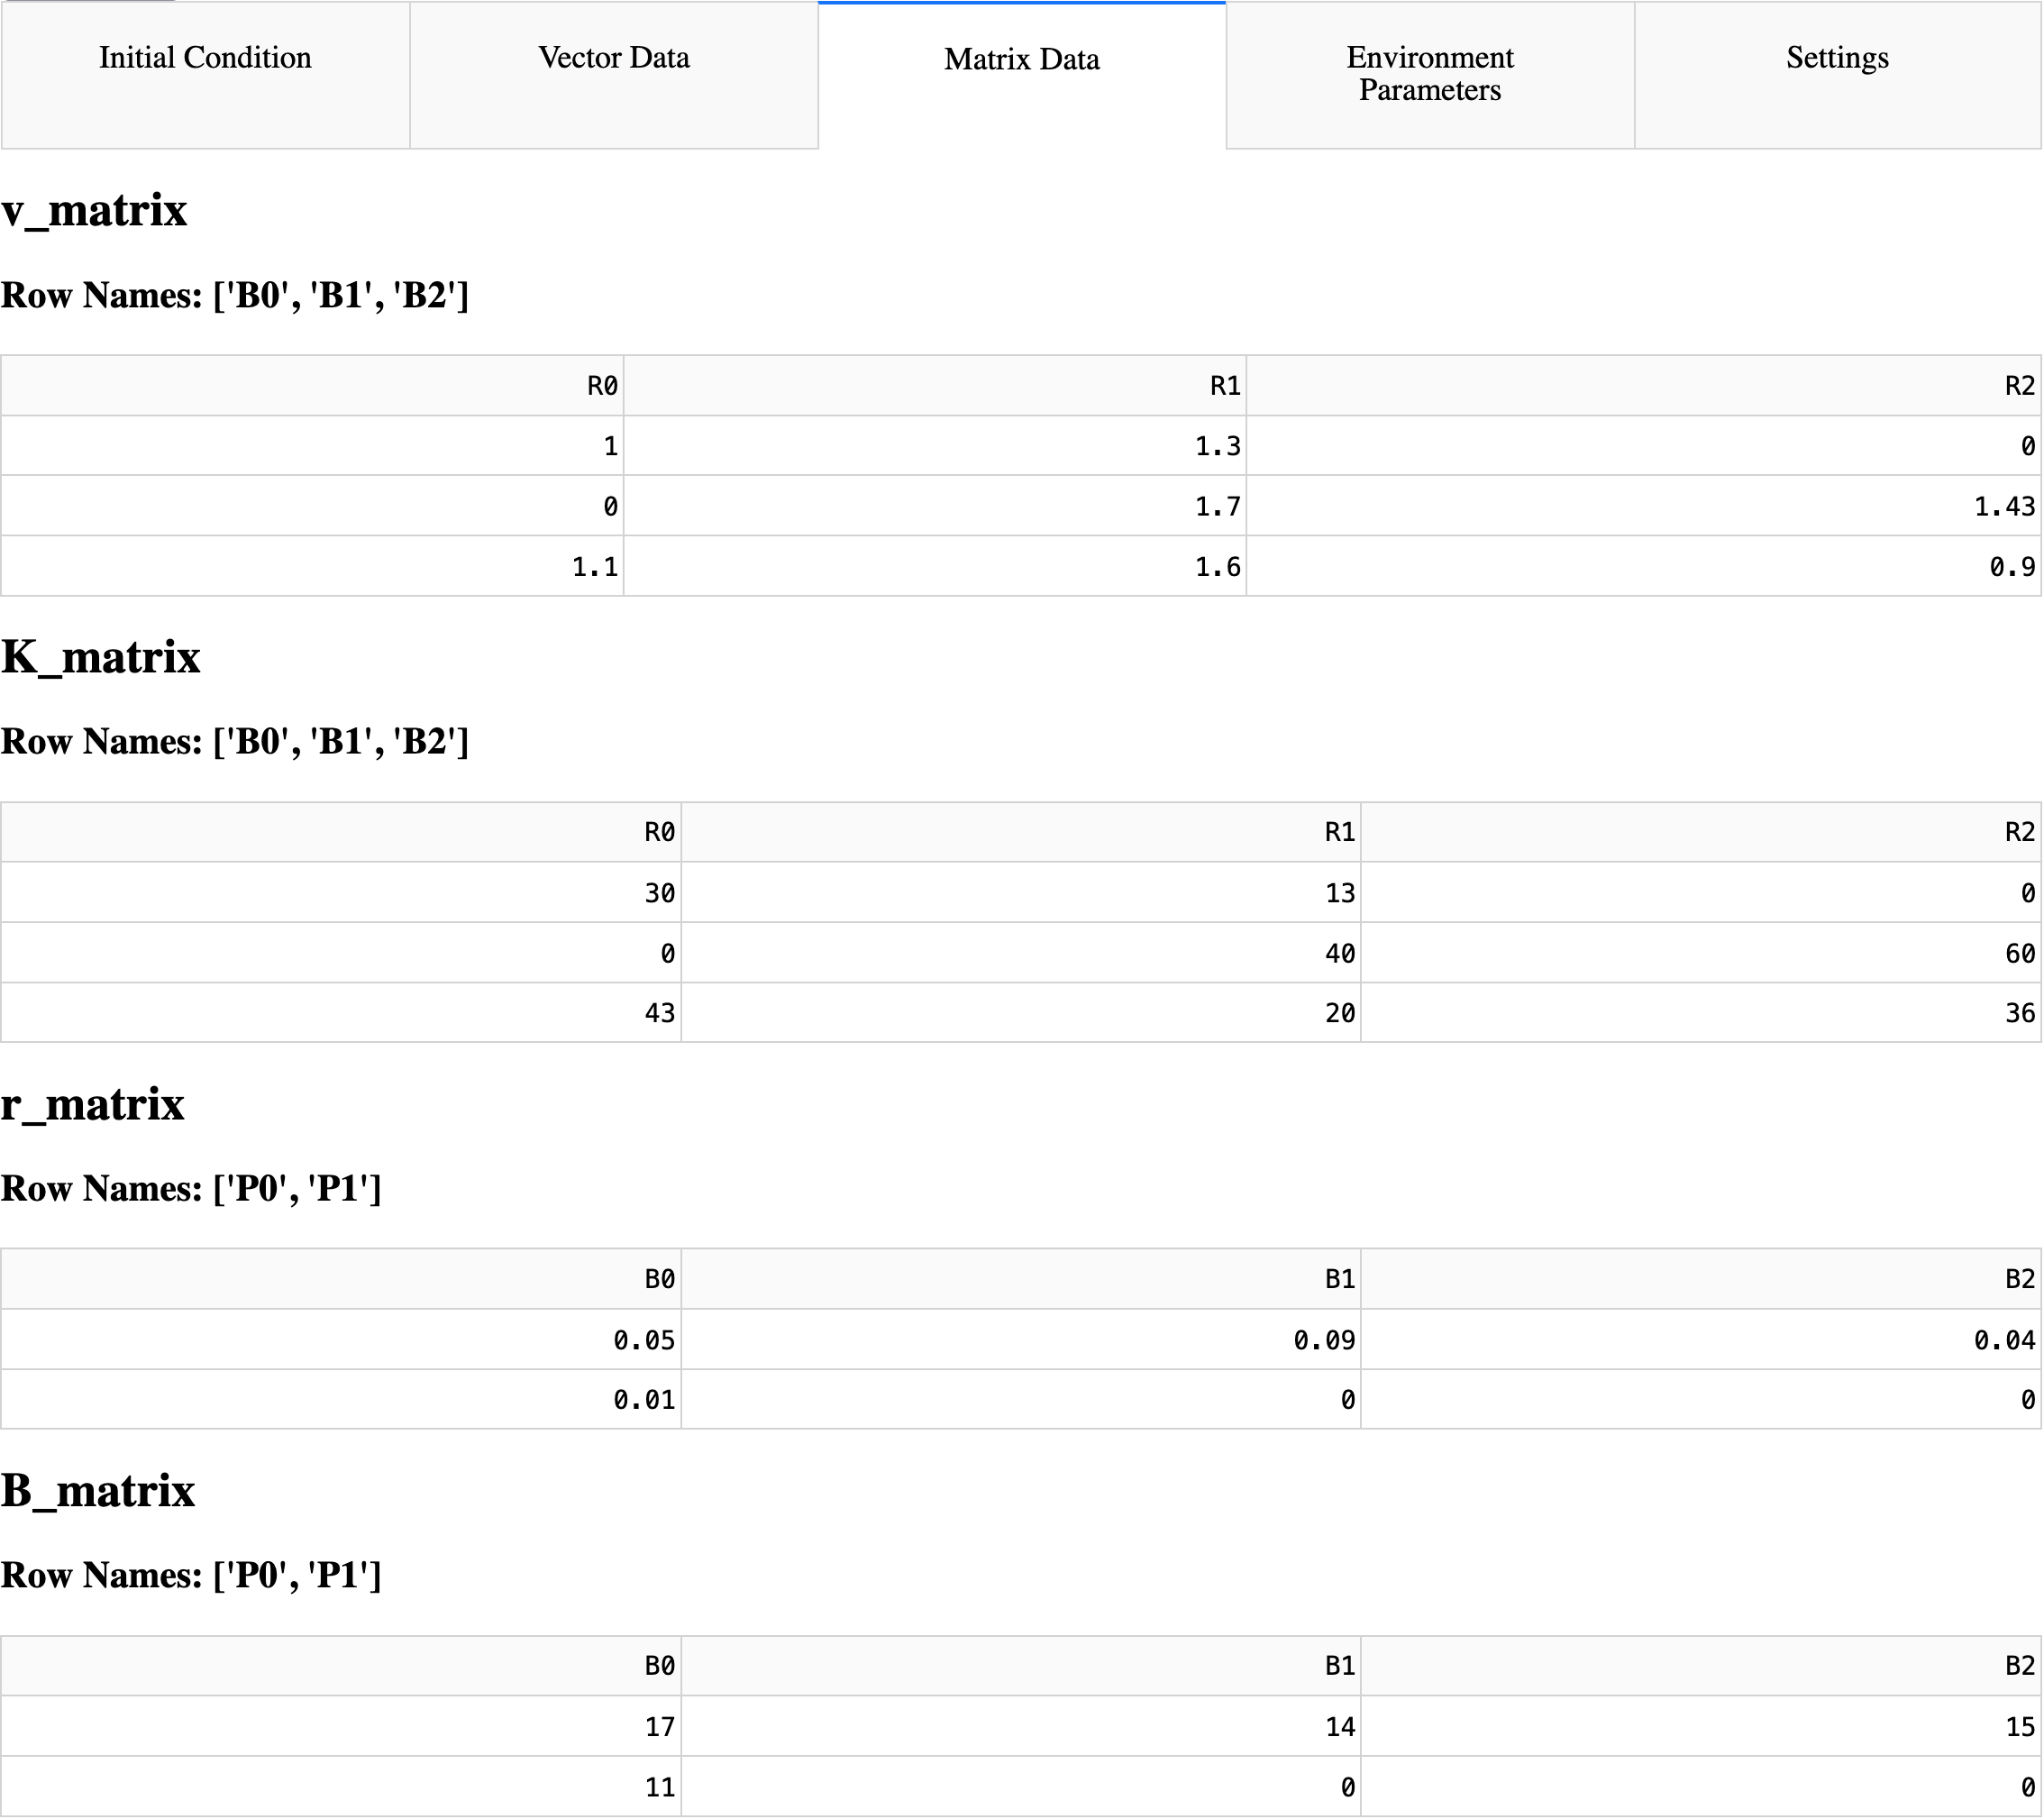
\includegraphics[width=1\linewidth]{Screenshots/DashboardSettings/initial_matrix_settings.png}
    \caption{
        The panel where the user can edit the attributes for a given attribute name. 
        This version is specifically used to represent the attributes that are associated with edges between agents, and are represented as a matrix. 
        The rows and columns of each table show for which agent the value corresponds to. 
        Due to limitations with Dash datatables, the row names can't explicitly be labelled, however text above the table shows the row names. 
        A copy of this data is sent to the solver. 
    }
    \label{fig:ss:ds:matrix}
\end{figure}
\begin{figure}
    \centering
    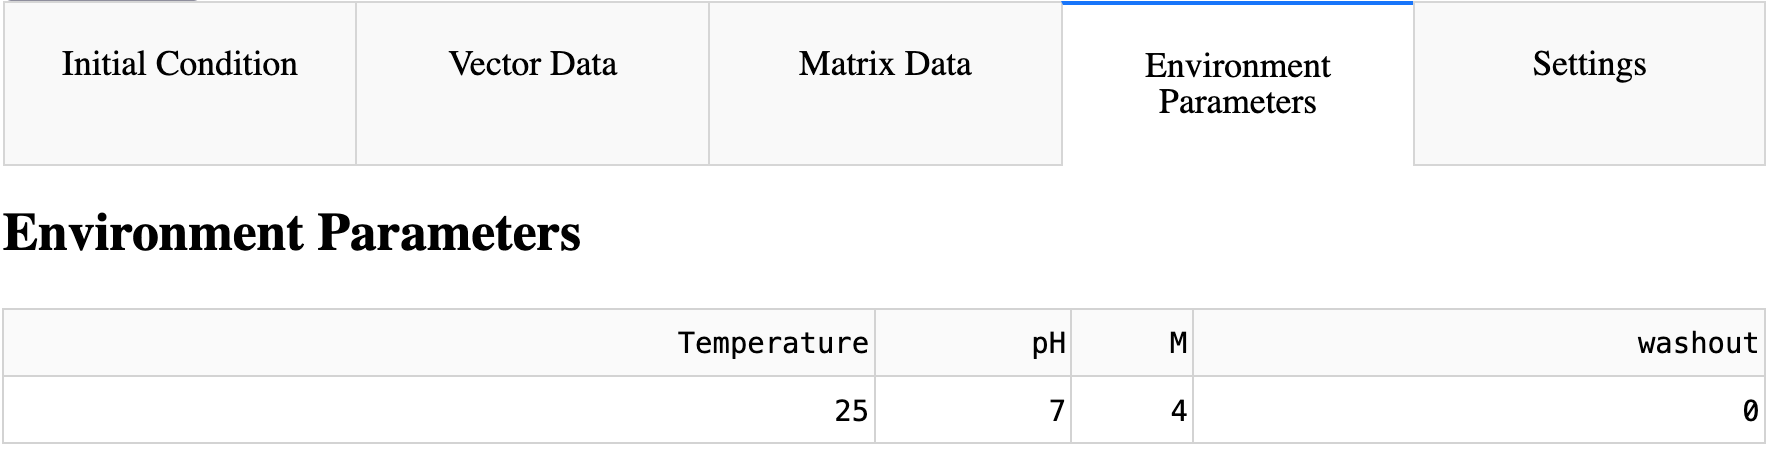
\includegraphics[width=1\linewidth]{Screenshots/DashboardSettings/initial_environment_settings.png}
    \caption{
        The panel where a user can edit the edge attributes the environment settings. 
        Each column represents a single environment parameter. 
        A copy of this data is sent to the solver.
    }
    \label{fig:ss:ds:environment}
\end{figure}
\begin{figure}
    \centering
    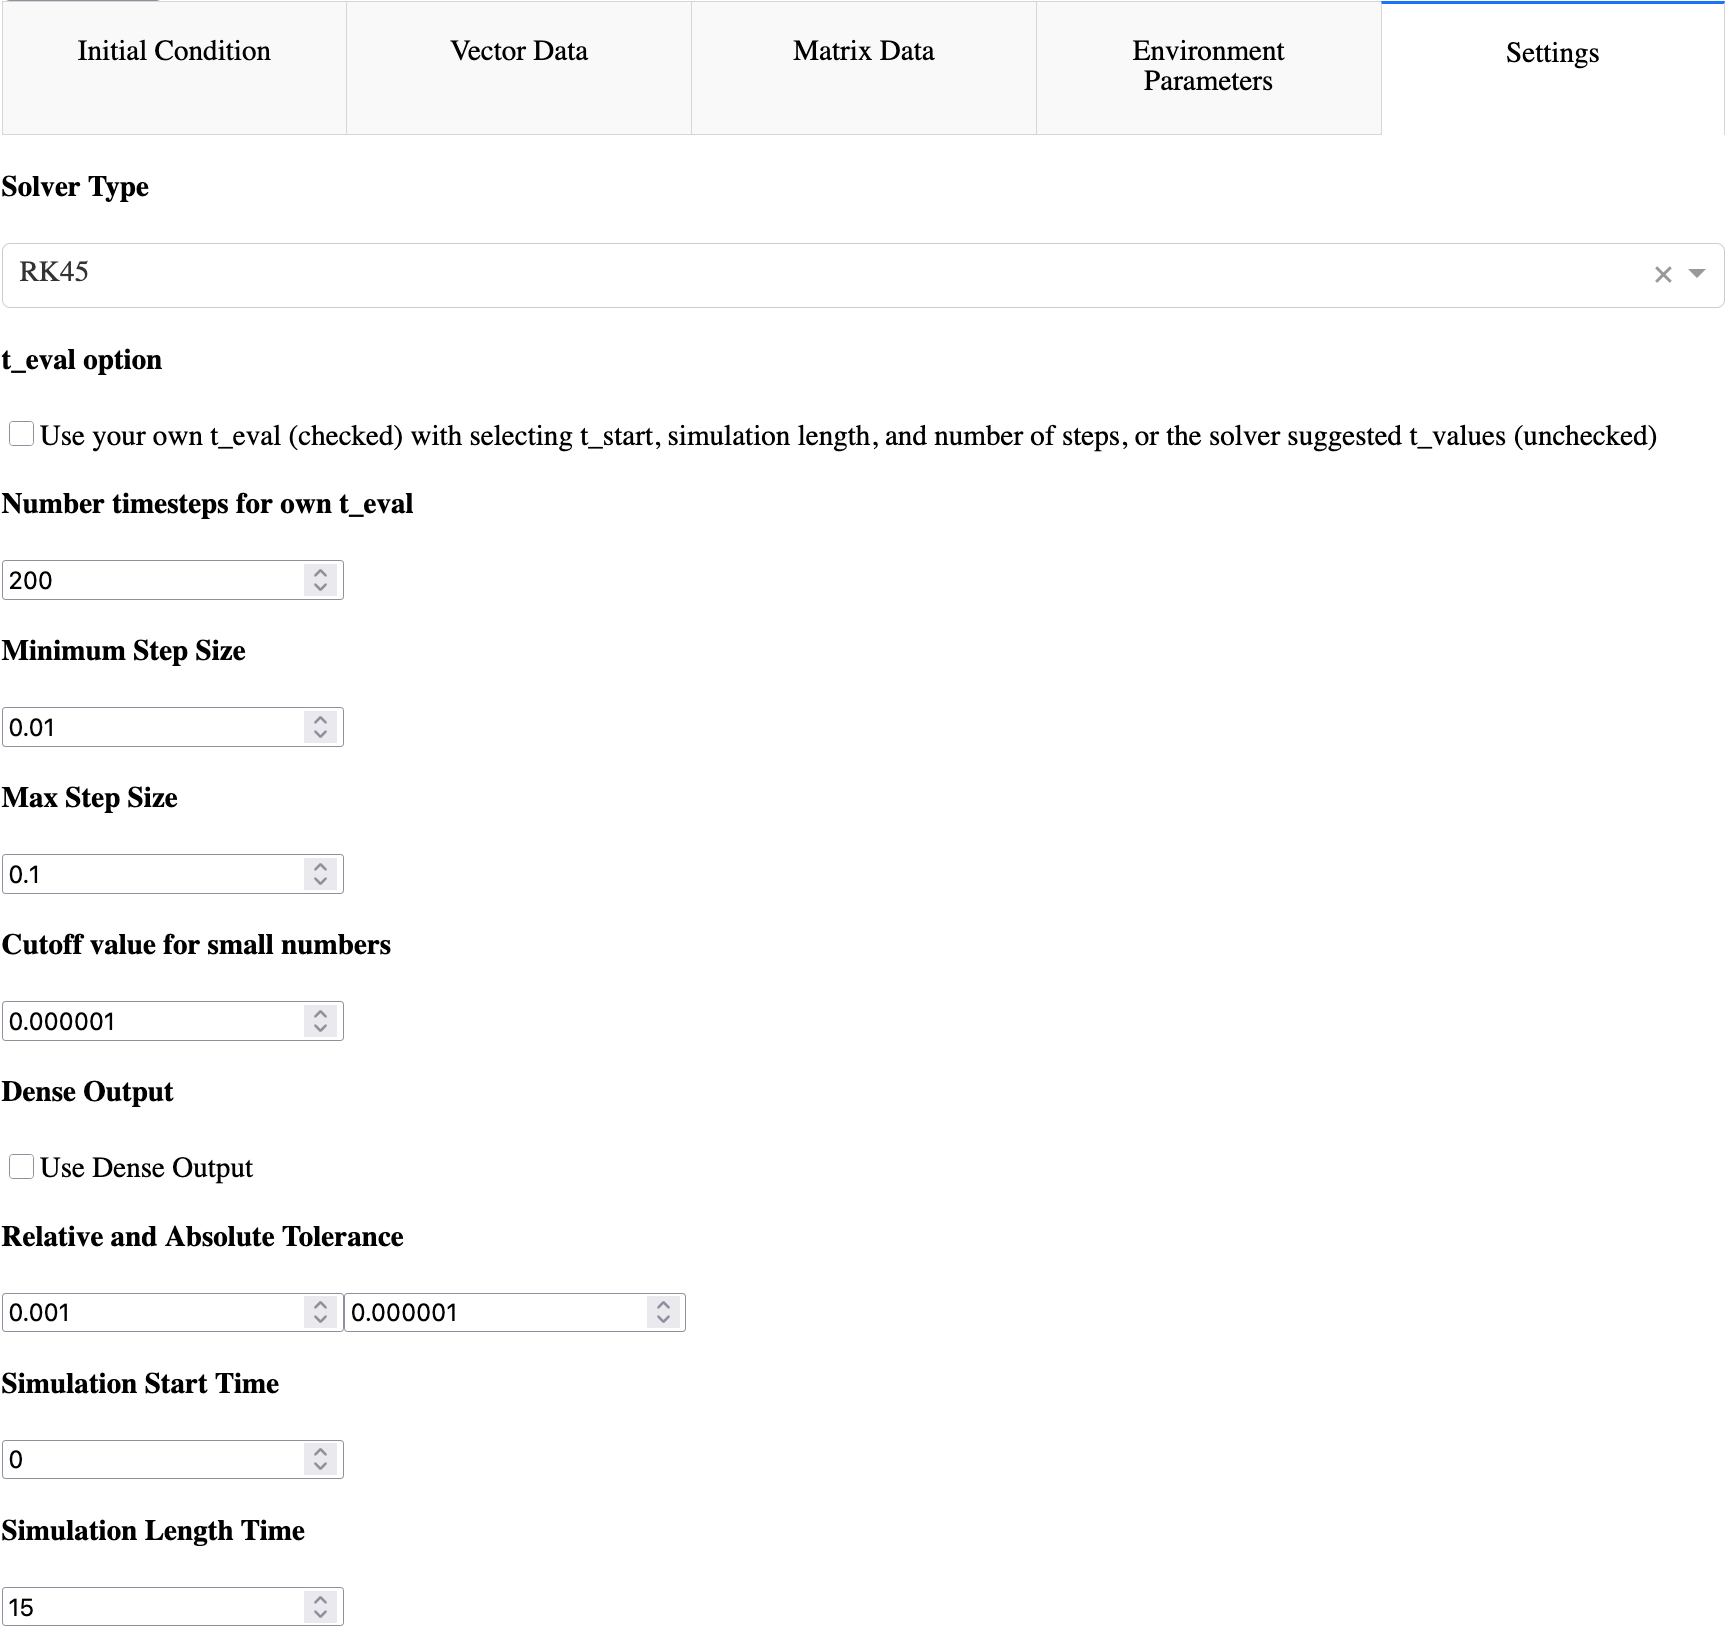
\includegraphics[width=1\linewidth]{Screenshots/DashboardSettings/initial_settings_settings.png}
    \caption{
        The panel where a user can edit the settings of the solver. 
        Various options exist, such as solver type, cutoff value for small values, or tolerances of the solver. 
        A copy of this data is not sent to the solver. 
        The user needs to save the settings, while for the other panels the user does not need to save the changes. 
    }
    \label{fig:ss:ds:settings}
\end{figure}

\subsection{Advanced Visualization and Analysis}
In the advanced analysis section, the user can run different analysis methods to gain a greater understanding of the model. 
The visualizations only support a $1 \times 1\times 1$ model, in order to make the analysis easier for the user, and to make it easier to analyze the visualization. 
These advanced visualizations were created with the mind of understanding a simple network. 
There are five different analysis and visualization methods, and one system where the user can run a large simulation on the whole network and receive an output file containing the raw simulation file data. 
The raw data is stored as a \textit{parquet} file, a tabular-like dataformat, which when combined with Dask (note: not Dash), allows for querying of the data similarly to Pandas. 
Parquet with Dask offers superior performance and data storage solutions that Pandas can't offer. 
Once queried, the user can create their own graphs and plots as they have access to the parameter values used and the raw simulation data. 
\subsubsection{Serial Transfer}
Serial transfer is a method employed by bacteriologist where after a set amount of time, the bacteriologist pipettes a specified amount of media (for example 10ml of liquid) containing bacteria and  nutrients, possibly with phages, and transfers the old media into a solution containing new media. 
At this stage, the bacteriologist can introduce new agents, or re-introduce agents if the agent population or concentration has died out. 
However, usually only resources are added during the transfer process. 
An example would be an experiment starts with 50ml of solution. 
The experiment runs for 24 hours before 5ml is removed. 
Researchers can run various tests, such as using optical density measurements to assess bacterial density in the solution or employing a mass spectrometer to determine the concentration of the resources. 
The 5ml is then re-added to a new solution of 45ml containing fresh resources. 
The effect that this has is tit creates a sort of artificial stable point. 
As the bacteria grow, they consume the resources found in the solution. 
However eventually the resources run out, and the bacteria die out due to a lack of nutrients. 
By introducing new nutrients at set time intervals, the bacteria can regrow and exhibit a semi-stationary behavior. 
\newline 

The implementation of serial transfer is slightly different. 
A user can select a number which will divide the population count of the agents by that number. 
Then the program takes the initial condition values defined for the nutrients the initial condition in \ref{sec:editing_network_and_parameter_values} and adds those values to the nutrients respectively. 
By selecting a checkbox, the values as defined in the initial condition box for phages and bacteria in \ref{sec:editing_network_and_parameter_values} can optionally be added as well. 
As a concrete example, if at the end of a simulation, there are 120 resources remaining, 5000 bacteria, and 1000 phages, and the chosen serial transfer value is 15, then the ending resource, nutrient, and phage value is 8, 333.33, and 66.66 respectively. 
If the initial condition for the resources, bacteria, and phages are 500, 80, and 10 respectively, then if the checkbox is unchecked, the new population count will be 508, 333.33 and 66.66 respectively. 
If the checkbox is checked, the new population count will be 508, 413.33, and 76.66 respectively. 

\begin{figure}
    \centering
    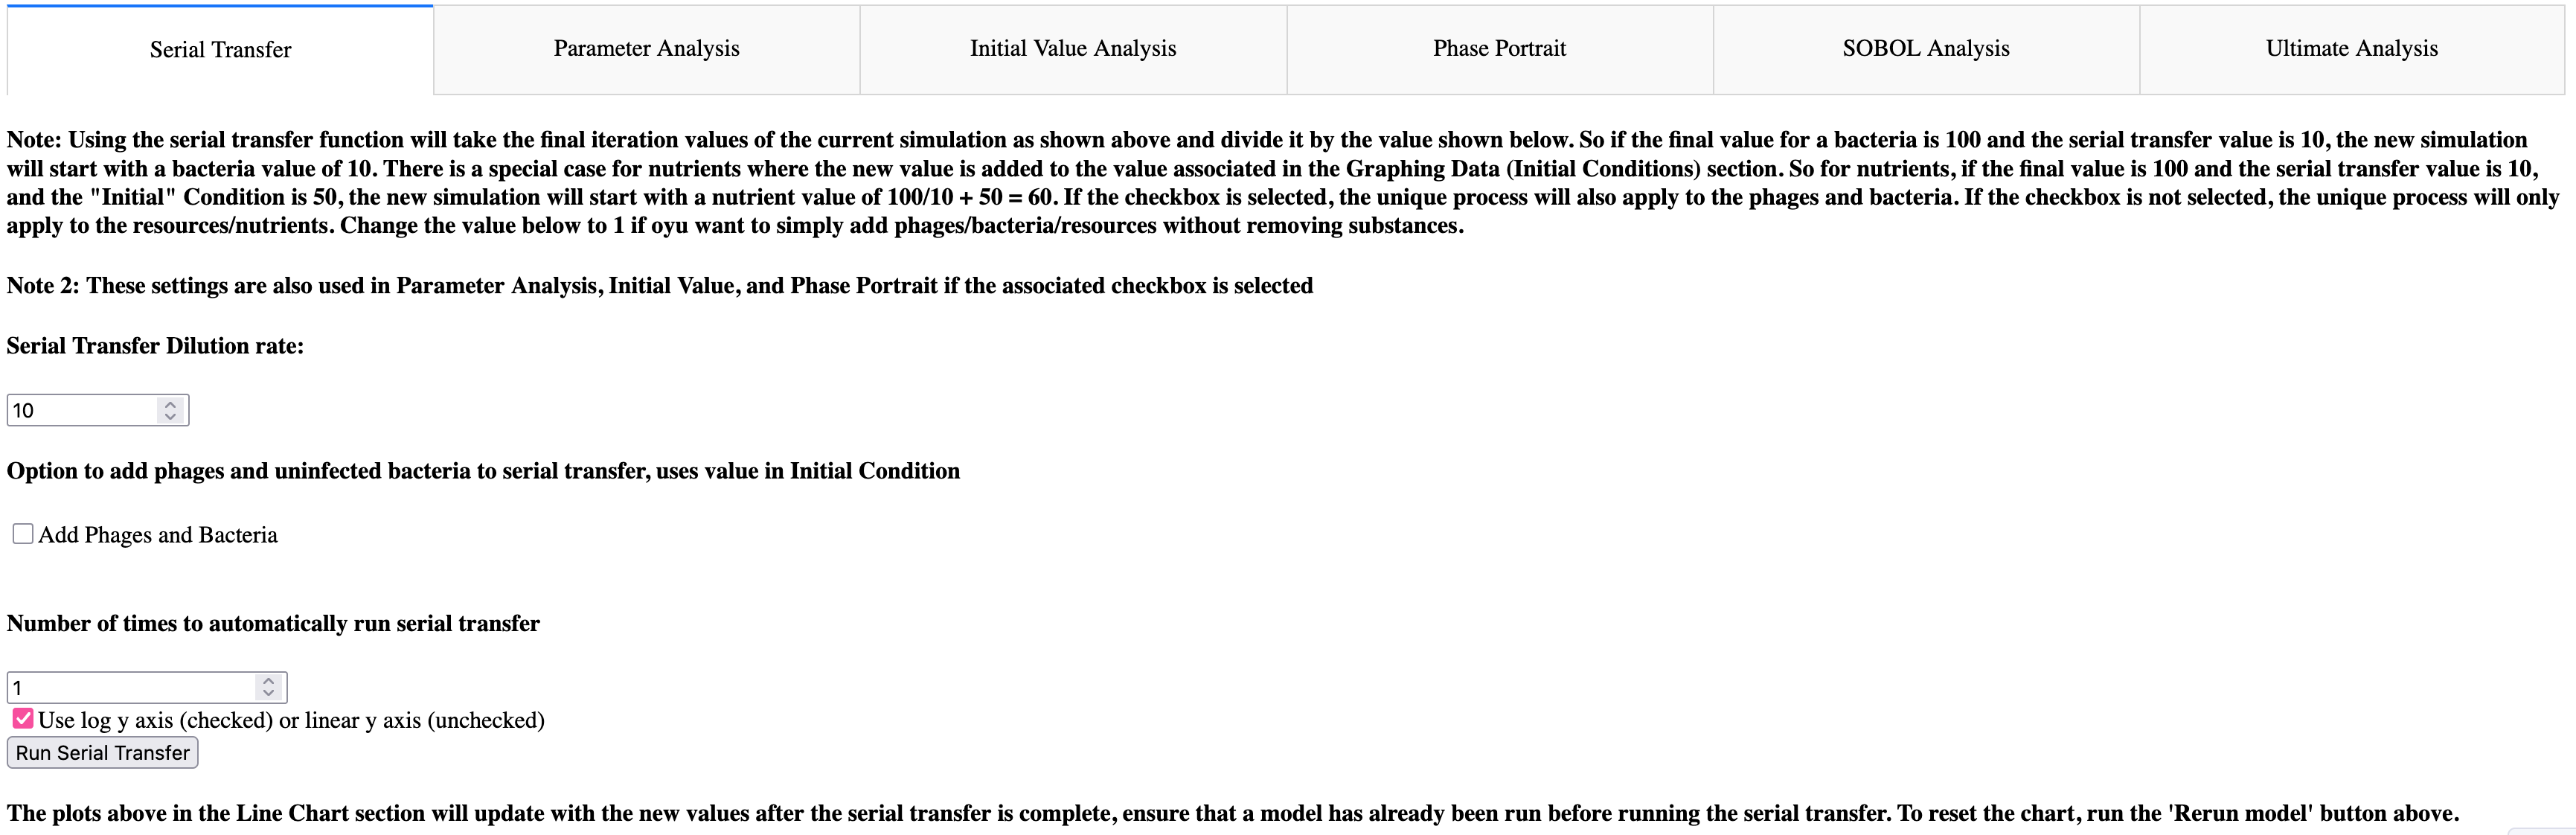
\includegraphics[width=1\linewidth]{Screenshots/AdvancedVisualization/serial_transfer_settings.png}
    \caption{
        The section where the user can set up the serial transfer. To adjust the values added, the user would need to edit the initial condition values. 
    }
    \label{fig:ss:av:serial_transfer_settings}
\end{figure}
\begin{figure}
    \centering
    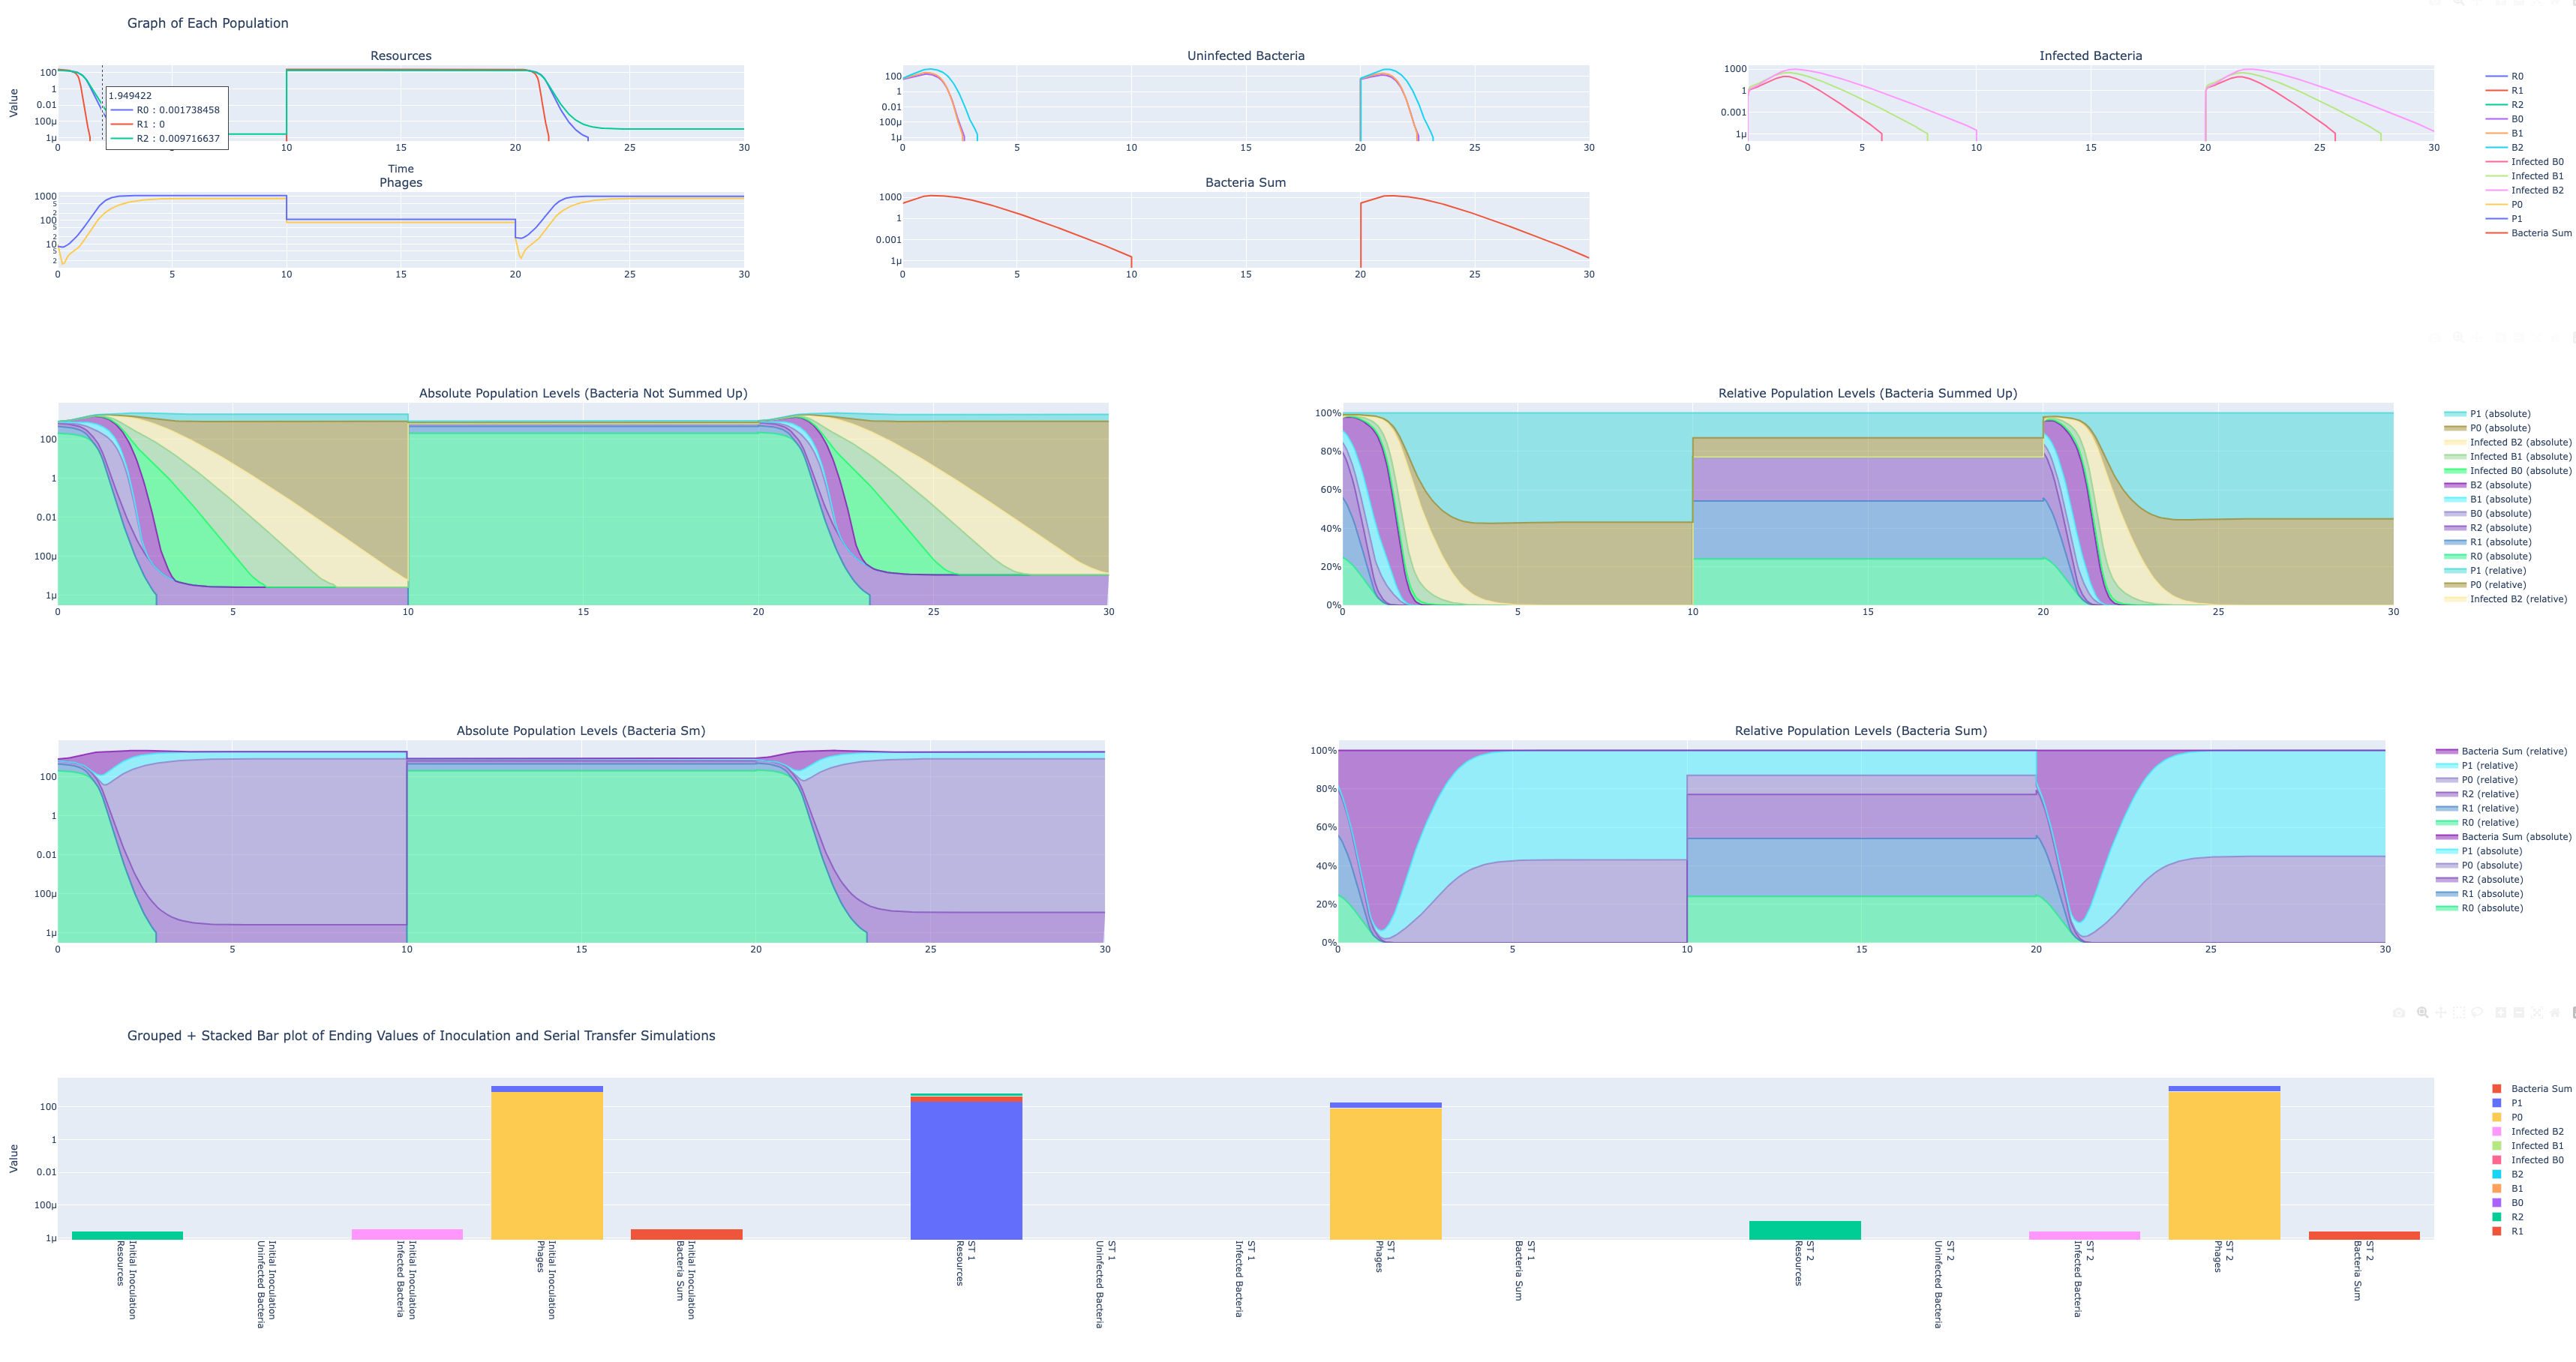
\includegraphics[width=1\linewidth]{Screenshots/AdvancedVisualization/serial_transfer_run2_with_p_b.png}
    \caption{
        Running the serial transfer updates the plot at the top of the page. 
        The simulation initially ran for $t=10$, and completed two serial transfers with a dilution rate of 10. 
        The first transfer was completed without adding new phages and bacteria. 
        The second transfer was done with adding new phages and bacteria. 
        The R1 (red) and R0 (purple) resource died out at $t=1.5$ and $t=2.8$ but are reintroduced at $t=10$ as part of the serial transfer process. 
        All bacteria become infected and die out before or at $t=10$. 
        At $t=10$ the phages have a value of roughly 818 and 1078 pre-serial transfer, and have a value of 81.8 and 107.8 post serial transfer. 
        At $t=20$, a second serial transfer occurs where the bacteria were reintroduced to the system, and more phages were added to the existing population. 
        The stacked line plots show the absolute and relative distribution of different population groups. 
        The stacked bar chart at the bottom shows the final population count of each agent group type at the end of each serial transfer. 
        It might not always be feasible to experimentally determine the population count at each timestep in a lab, hence this graph can be used as a replacement to show the population count at serial transfer time. 
    }
    \label{fig:ss:av:serial_transfer_run2_with_p_b}
\end{figure}

\subsubsection{Parameter Analysis}
The parameter analysis allows the user to choose two parameters and individually run the model with the varying input values. 
The values that can be tested and changed include all initial condition values, vector and matrix data, and environmental data. 
As input, the user can select 2 parameters of choice. 
After the parameter name selection, the user can manually choose which parameter values they want to test or test a range of values equally spaced by selecting the number of values to test. 
Finally, the user can optionally run a serial transfer, where the serial transfer uses the settings found on the Serial Transfer tab. 
\begin{figure}
    \centering
    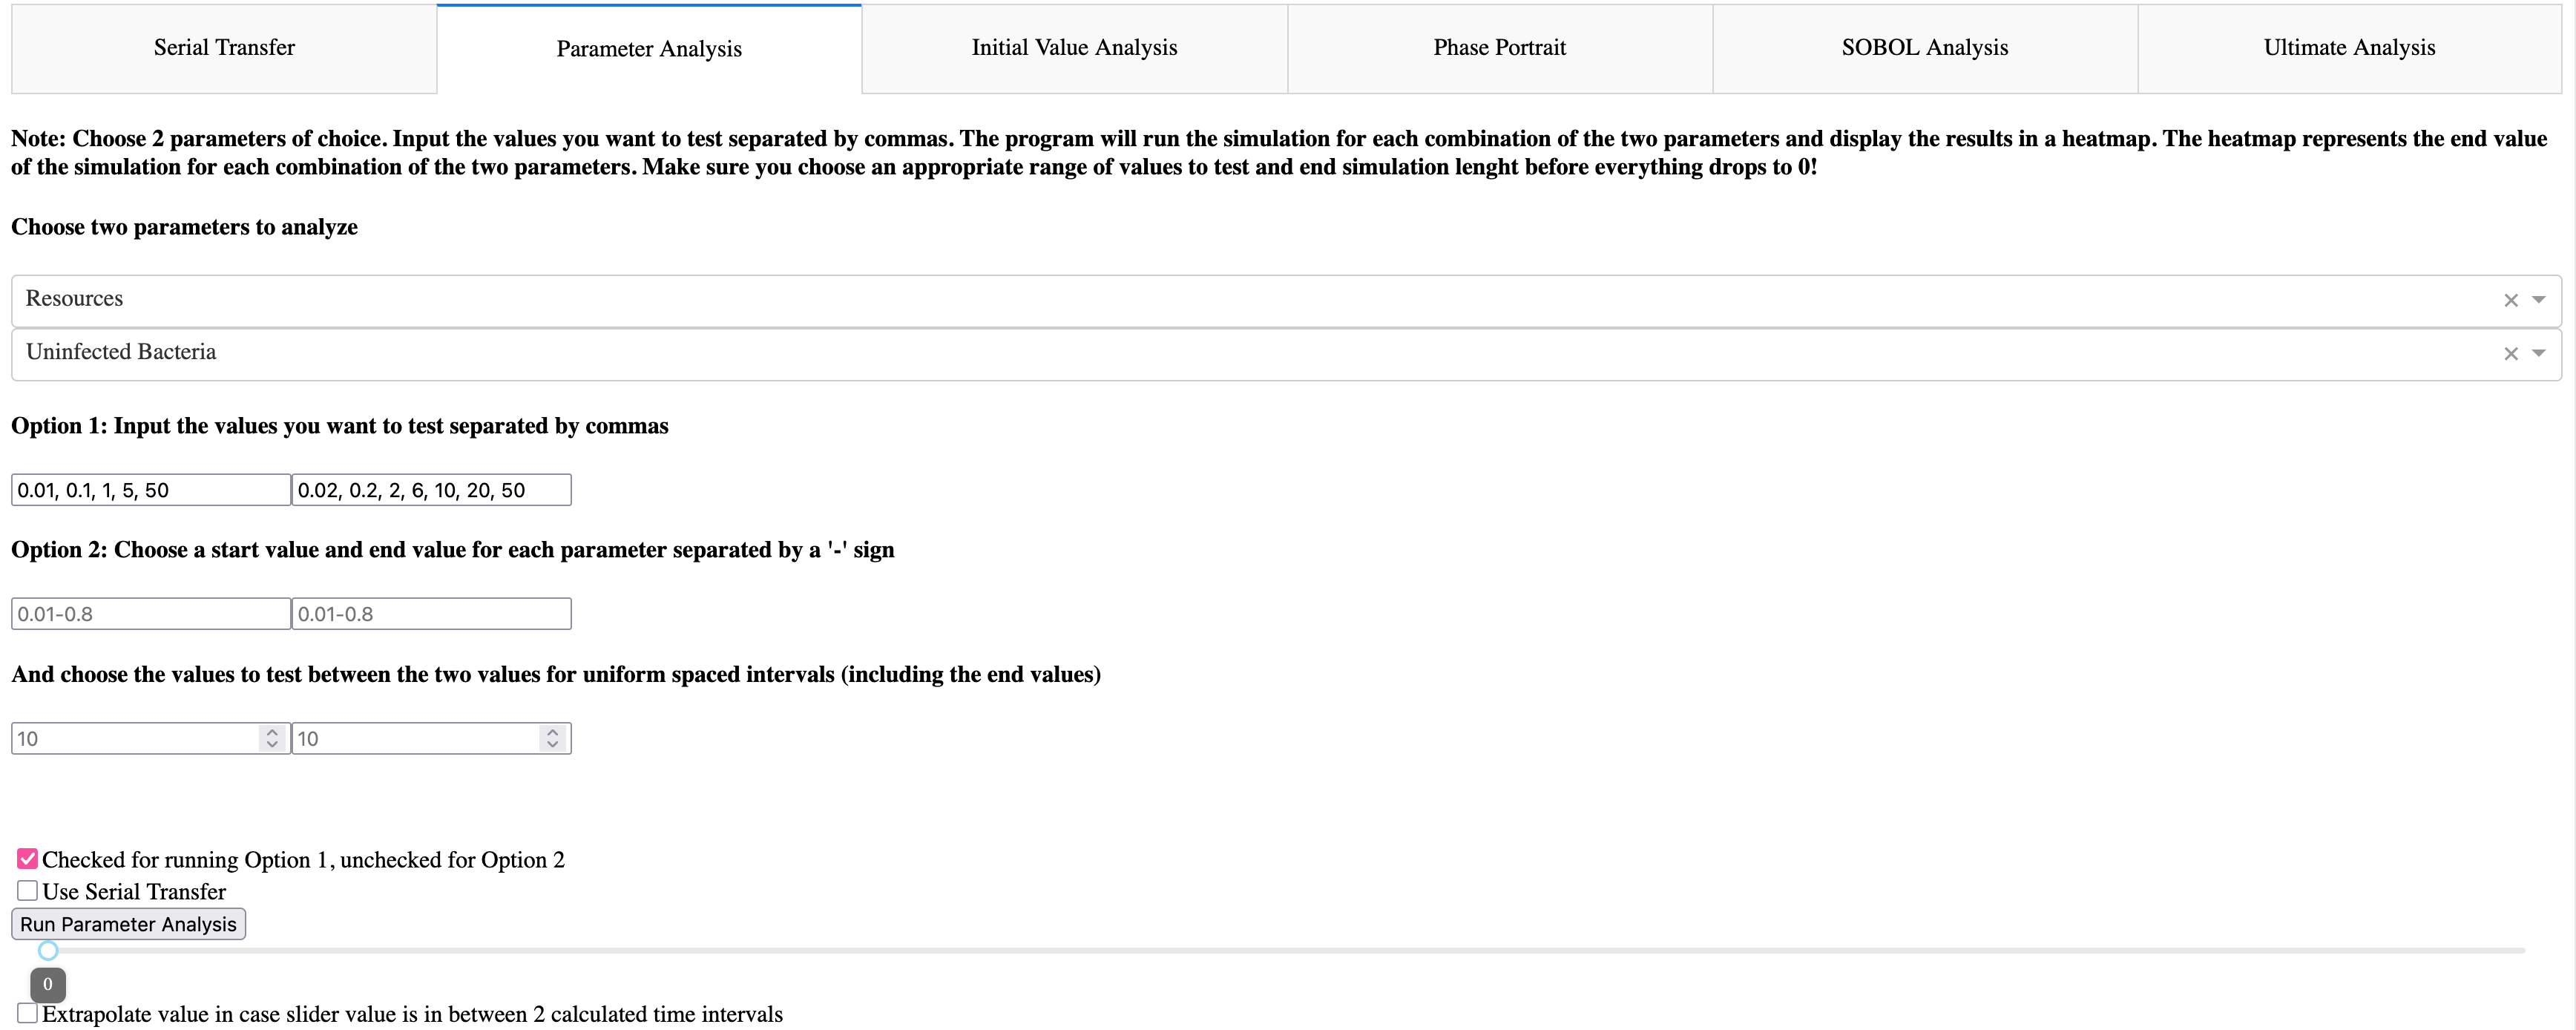
\includegraphics[width=1\linewidth]{Screenshots/AdvancedVisualization/parameter_analysis_settings.png}
    \caption{
        The user can choose two parameters to run, along with the values they want to test. 
        There is an option for a serial transfer, along with interpolating the values between the slider option. 
    }
    \label{fig:ss:av:parameter_analysis_settings}
\end{figure}
\begin{figure}
    \centering
    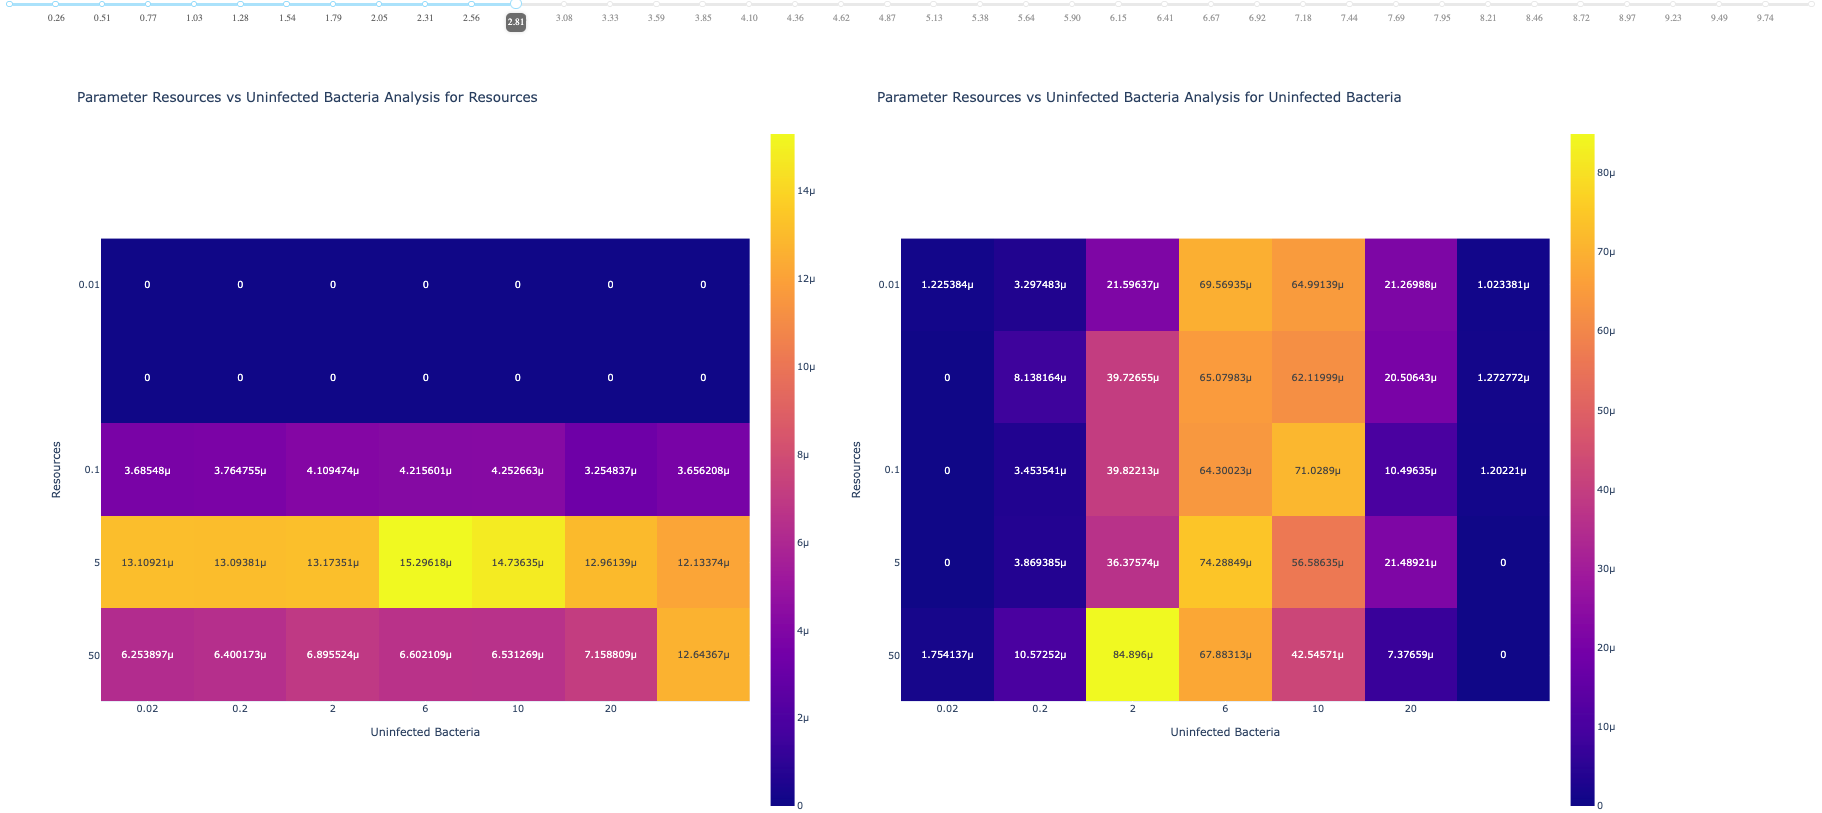
\includegraphics[width=1\linewidth]{Screenshots/AdvancedVisualization/parameter_analysis_run.png}
    \caption{
        An example run with the output. 
        A heatmap matrix is created for each agent type, with dimension of the input values. 
        Each box corresponds to each pair of parameter inputs, and shows the population count of the agent at that time, which can be changed by sliding the slider. 
        Note that the heatmap color range resets for each heatmap, and the units of the heatmap can reach to small numbers, such as $4\mu$. 
    }
    \label{fig:ss:av:parameter_analysis_run}
\end{figure}


\subsubsection{Initial Value Analysis}
The initial value analysis allows for the user to choose a single parameter and vary the value of that parameter. 

\begin{figure}
    \centering
    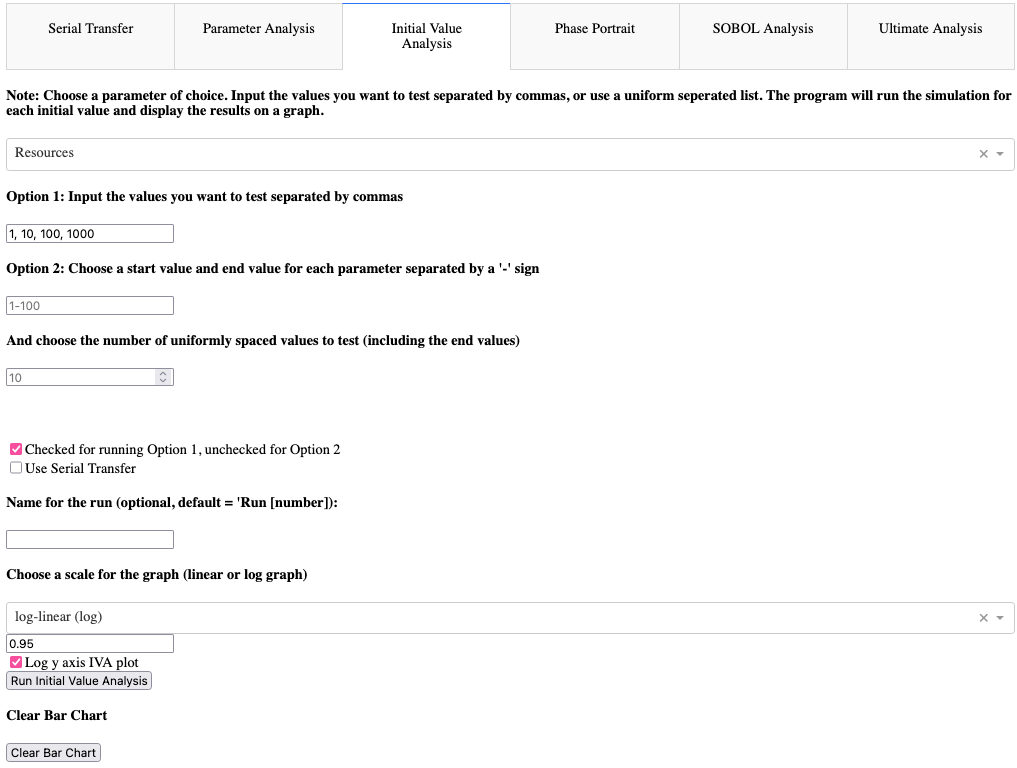
\includegraphics[width=1\linewidth]{Screenshots/AdvancedVisualization/initial_value_analysis_settings.png}
    \caption{
    }
    \label{fig:ss:av:initial_value_analysis_settings}
\end{figure}

\subsubsection{Parameter Space Slot}
\begin{figure}
    \centering 
    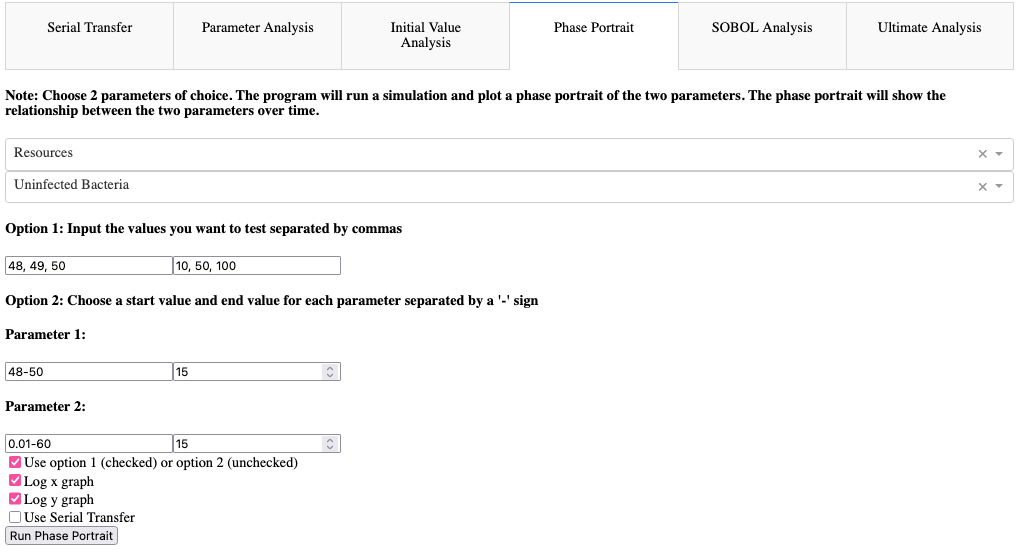
\includegraphics[width=1\linewidth]{Screenshots/AdvancedVisualization/parameter_space_settings.png}
    \caption{
        The user can select two starting values for the initial condition, but they can't choose vector, matrix, or environment settings due to the plot showing the development of agent populations against other agent populations. 
        As typical, the user can select their own values or auto-generate values between two values, as well as use a serial transfer option. 
        There is also an option to take the logarithm of the x and/or y axis. 
    }
    \label{fig:ss:av:phase_portrait_settings}
\end{figure}
\begin{figure}
    \centering 
    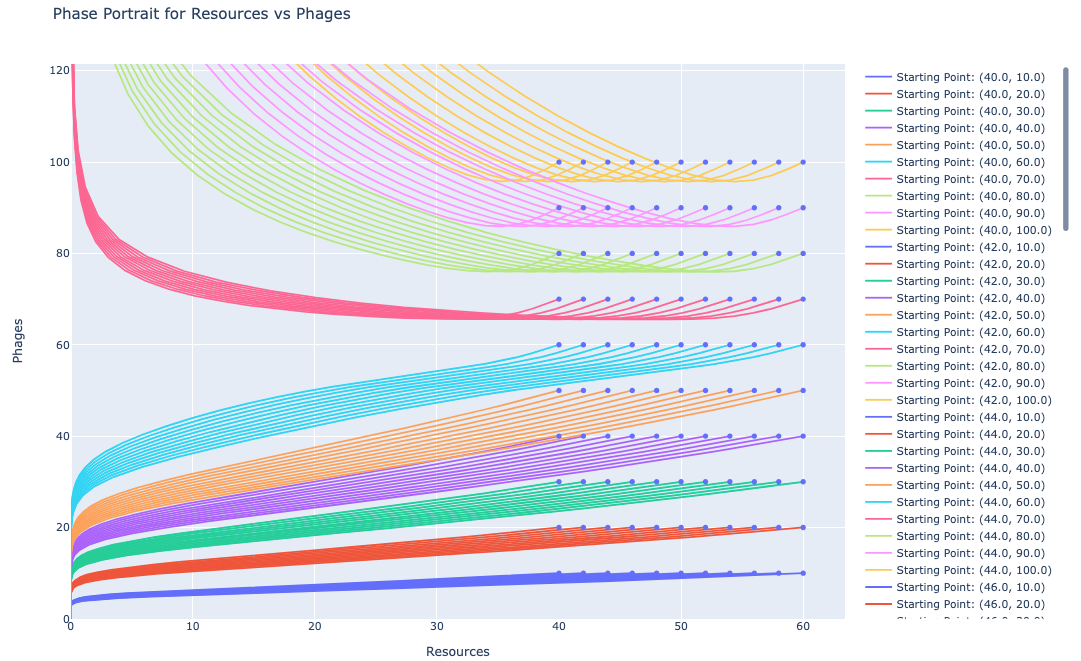
\includegraphics[width=1\linewidth]{Screenshots/AdvancedVisualization/parameter_space_run.png}
    \caption{
        An example run of a parameter space plot. 
        Resources are plotted against phages, with a high washout rate of $0.05$ explaining why the phage population is decreasing. 
        For initial phage population of 60 and less, the phages “die out” due to the washout rate, while for an initial population count of 70 and higher the phages are able to proliferate. 
        There is an initial population decrease due to the washout, but after the infected bacteria start to die out and release new phages, the population can grow. 
    }
    \label{fig:ss:av:phase_portrait_run}
\end{figure}

\subsubsection{SOBOL Analysis}
SOBOL analysis, a variance-based sensitivity analysis, is a method that allows a user to quantify how important an input parameter has on a measured aspect of the output by changing the parameter values of the model and measuring the change in model output. 
SOBOL quantifies how much variance in the output can be attributed to a specific parameter and cna measure the effect of global, first, and second order sensitivity.  
When a model is viewed as a black-box model, the model can be seen as a function $Y=f(X)$, where $X$ is an input vector of $d$ elements, and $Y$ is a univariate model output. 
$X$ is assumed to be independently and uniformly distributed within a hypercube $X_i \in [0, 1]$ for $i=1, \dots d$. 
The first order sensitivity measures the output variance of the main affect of parameter $X_i$. 
Measuring the effect of varying $X_i$ averaged over other input parameters, and standardized to provide a fractional contribution to the overall output variance. 
The first order sensitivity is described as 
\[
    S_i = \frac{V_i}{Var(Y)}
\] where $V_i = Var_{X_i}(E{X_{\sim i}}(Y|X_i))$ and where $X_{\sim i}$ represents all the parameters that are not $X_i$. 
\newline

The second order index measures the impact of input $X_i$ interacting with $X_j$. For many inputs, this becomes unwieldy to analyze. 
The global sensitivity is used to analyze the global sensitivity without evaluating $2^d-1$ indices, and measures the contribution to the output variance of $X_i$, including all variance due to $X_i$s interaction with other variables. 
\[
    S_{T_i} = \frac{E_{X_{\sim i}}(Var_{X_i}(Y|X_{\sim i}))}{Var(Y)} = 1 - \frac{Var_{X_i}(E_{X_i}(Y|X_{\sim i}))}{Var(Y)}
\]
SOBOL can analyze various univariate outputs. 
This could be either the average value of an agent population, the variance in population count, the time at the peak of an agent count, the final population value, etc. 
\begin{figure}
    \centering
    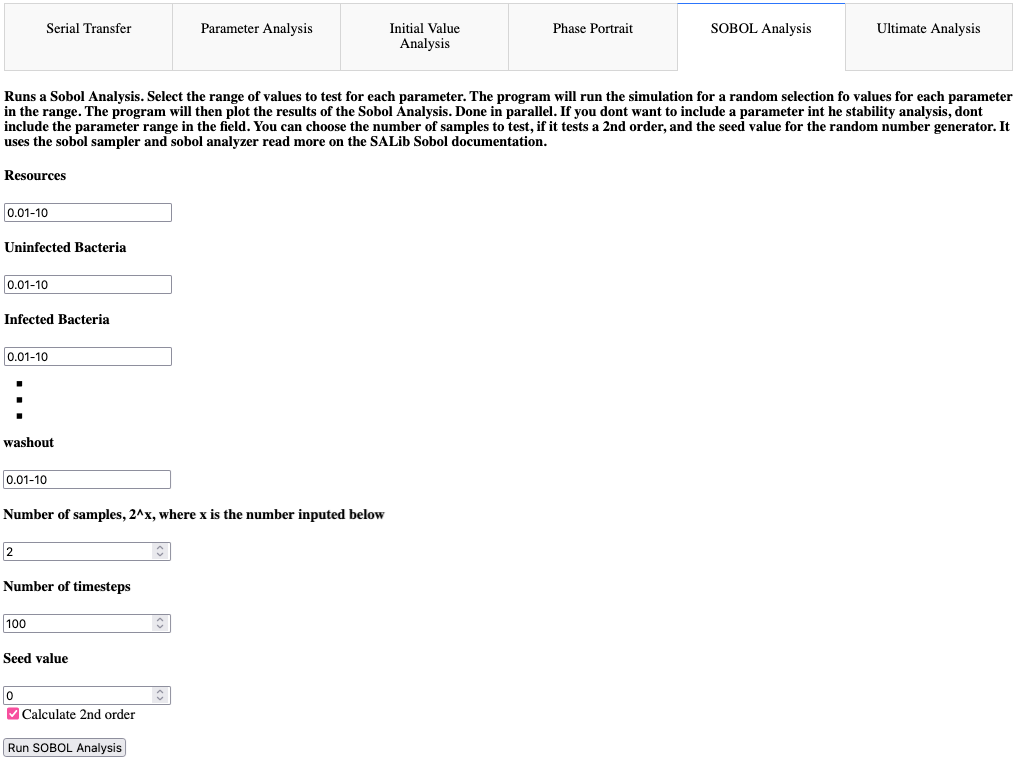
\includegraphics[width=1\linewidth]{Screenshots/AdvancedVisualization/SOBOL_analysis_settings.png}
    \caption{
		For each parameter, the user can choose a range of values that SOBOL will use to test and analyze. 
		If no values for a parameter are inputted, then the parameter is not included in the analysis. 
		The user then needs to select the number of samples to run. 
        The larger the number, the more accurate the results, but more simulations would need to be run. 
        If the user wants to analyze the second order interactions, then the model will run the system $N(2D+2)$ times with the randomly sampled input values, where $N$ is a multiple of 2, and $D$ is the number of parameters being tested. 
        Otherwise, if 2nd order is not chosen, the model is run $N(D+2)$ times. 
        As each run can produce different time data of varying length, the number of timesteps has to be fixed by the user. 
        Due to the randomness of the sampling method, a seed value can be provided to ensure repeatable results. 
    }
    \label{fig:ss:av:SOBOL_analysis_settings}
\end{figure}

\subsubsection{Ultimate Analysis}
The Ultimate Analysis section does not produce any visualizations or analysis, but instead allows for the user to define which initial conditions and parameter values they want to run a simulation on. 
The solver will iterate over every single parameter input possibility and save the results in a \textit{.parquet} file. 
Similarly to the other sections, the user can specify a start and end value, along with the number of values to generate evenly spaced within that range, including both the start and end values. 
\newline 
Using Dask and the saved \textit{.parquet}, the user can query for specific runs, for example runs where a parameter value was greater than 0.05, and use the simulation data to create their own plots. 
\begin{figure}
    \centering
    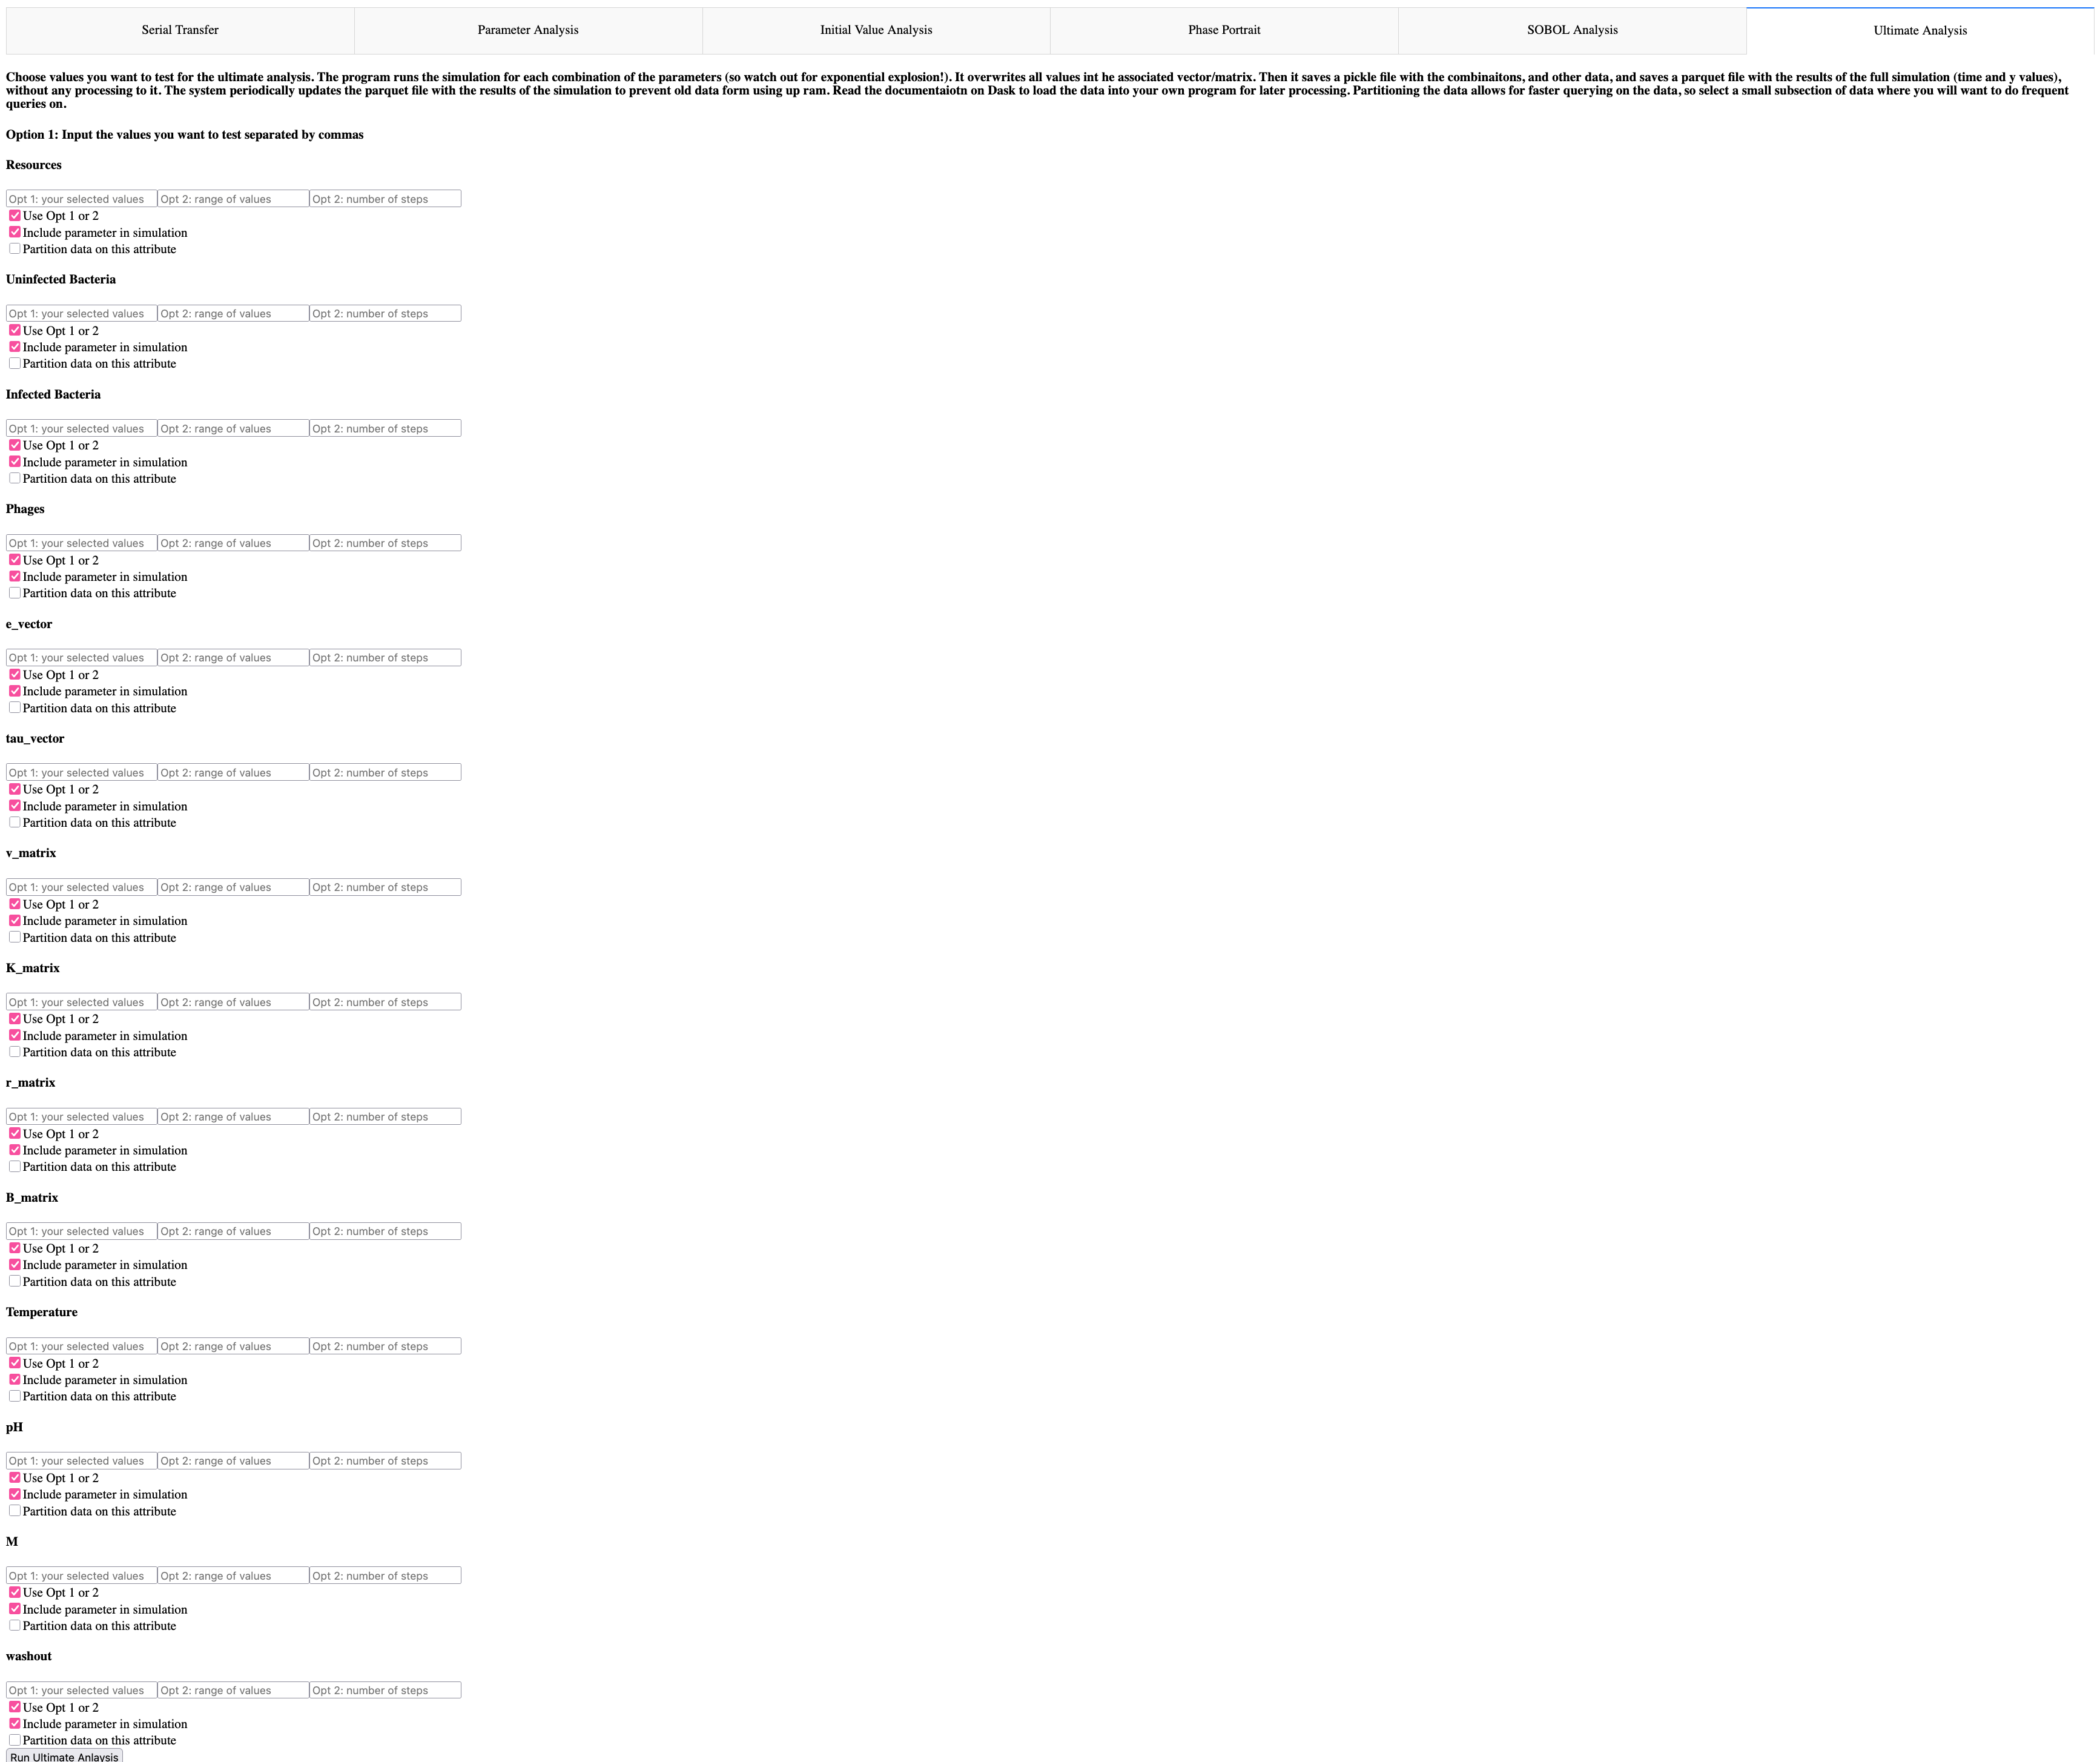
\includegraphics[width=1\linewidth]{Screenshots/AdvancedVisualization/ultimate_analysis_settings.png}
    \caption{
        The section where a user can start an ultimate analysis, where they provide the values they want to test, and run the simulations. 
        As an output, the user receives a $.parquet$ file containing the parameter values that were changed for that specific and the $t$ and $y$ values for that specific run. 
        A pickle file of a dictionary containing information on that run such as the parameter names and values chosen, the original graph data, and original parameter values. 
    }
    \label{fig:ss:av:ultimate_analysis_settings}
\end{figure}
